% !TeX spellcheck = hu_HU
% !TeX encoding = UTF-8
% !TeX program = xelatex
% TODO Change language to en_GB (recommended) or en_US for English documents
\documentclass[11pt,a4paper,oneside]{report}             % Single-side
%\documentclass[11pt,a4paper,twoside,openright]{report}  % Duplex

\usepackage{ifxetex}
\ifxetex
  \usepackage{fontspec}
\else
  \usepackage[T1]{fontenc}
  \usepackage[utf8]{inputenc}
  \usepackage[lighttt]{lmodern}
\fi

\usepackage[english,magyar]{babel} % Alapértelmezés szerint utoljára definiált nyelv lesz aktív, de később külön beállítjuk az aktív nyelvet.

%\usepackage{cmap}
\usepackage{amsfonts,amsmath,amssymb} % Mathematical symbols.
\usepackage[ruled,boxed,resetcount,linesnumbered]{algorithm2e} % For pseudocodes.
\usepackage{booktabs} % For publication quality tables for LaTeX
\usepackage{graphicx}

%\usepackage{fancyhdr}
%\usepackage{lastpage}

\usepackage{anysize}
%\usepackage{sectsty}
\usepackage{setspace} % For setting line spacing

\usepackage[unicode]{hyperref} % For hyperlinks in the generated document.
\usepackage{xcolor}
\usepackage{listings} % For source code snippets.

\usepackage[amsmath,thmmarks]{ntheorem} % Theorem-like environments.

\usepackage[hang]{caption}

\singlespacing

\newcommand{\selecthungarian}{
	\selectlanguage{magyar}
	\setlength{\parindent}{2em}
	\setlength{\parskip}{0em}
	\frenchspacing
}

\newcommand{\selectenglish}{
	\selectlanguage{english}
	\setlength{\parindent}{0em}
	\setlength{\parskip}{0.5em}
	\nonfrenchspacing
	\renewcommand{\figureautorefname}{Figure}
	\renewcommand{\tableautorefname}{Table}
	\renewcommand{\partautorefname}{Part}
	\renewcommand{\chapterautorefname}{Chapter}
	\renewcommand{\sectionautorefname}{Section}
	\renewcommand{\subsectionautorefname}{Section}
	\renewcommand{\subsubsectionautorefname}{Section}
}

\usepackage{pdfpages}
\usepackage{hyperref}

%TODO Set the main variables
\newcommand{\vikszerzoVezeteknev}{Deim}
\newcommand{\vikszerzoKeresztnev}{Péter Pál}
\newcommand{\vikkonzulensA}{Semeráth Oszkár} % Első konzulens neve
\newcommand{\vikkonzulensB}{} % Második konzulens neve; hagyd üresen, ha egy konzulensed van.
\newcommand{\vikcim}{Általános célú szerkesztőfelület\\ parciális modellekhez} % Cím
\newcommand{\viktanszek}{\bmemit} % Tanszék
\newcommand{\vikdoktipus}{\bsc} % Dokumentum típusa (\bsc, \msc)

\input{include/tdk-variables}
\newcommand{\szerzoMeta}{\vikszerzoVezeteknev{} \vikszerzoKeresztnev} % egy szerző esetén
%\newcommand{\szerzoMeta}{\vikszerzoVezeteknev{} \vikszerzoKeresztnev, \tdkszerzoB} % két szerző esetén

%TODO Language configuration -- choose one
% Beállítások magyar nyelvű dolgozathoz
%--------------------------------------------------------------------------------------
% Elnevezések
%--------------------------------------------------------------------------------------
\newcommand{\bme}{Budapesti Műszaki és Gazdaságtudományi Egyetem}
\newcommand{\vik}{Villamosmérnöki és Informatikai Kar}

\newcommand{\bmemit}{Méréstechnika és Információs Rendszerek Tanszék}

\newcommand{\keszitette}{Készítette}
\newcommand{\konzulens}{Konzulens}

\newcommand{\bsc}{Szakdolgozat}
\newcommand{\msc}{Diplomaterv}
\newcommand{\bsconlab}{BSc Önálló laboratórium}
\newcommand{\msconlabi}{MSc Önálló laboratórium 1.}
\newcommand{\msconlabii}{MSc Önálló laboratórium 2.}

\newcommand{\pelda}{Példa}
\newcommand{\definicio}{Definíció}
\newcommand{\tetel}{Tétel}

\newcommand{\bevezetes}{Bevezetés}
\newcommand{\koszonetnyilvanitas}{Köszönetnyilvánítás}
\newcommand{\abrakjegyzeke}{Ábrák jegyzéke}
\newcommand{\tablazatokjegyzeke}{Táblázatok jegyzéke}
\newcommand{\irodalomjegyzek}{Irodalomjegyzék}
%\newcommand{\fuggelek}{Függelék}

\newcommand{\szerzo}{\vikszerzoVezeteknev{} \vikszerzoKeresztnev}

\newcommand{\selectthesislanguage}{\selecthungarian}

\bibliographystyle{huplain}

\def\lstlistingname{lista}

\newcommand{\appendixnumber}{6}  % a fofejezet-szamlalo az angol ABC 6. betuje (F) lesz

%\newcommand{\may}{\textit{May}}
%\newcommand{\var}{\textit{Var}}
%\newcommand{\abs}{\textit{Abs}}
%\newcommand{\ow}{\textit{OW}}
% Settings for English documents
%\input{include/thesis-en}

%--------------------------------------------------------------------------------------
% Page layout setup
%--------------------------------------------------------------------------------------
% we need to redefine the pagestyle plain
% another possibility is to use the body of this command without \fancypagestyle
% and use \pagestyle{fancy} but in that case the special pages
% (like the ToC, the References, and the Chapter pages)remain in plane style

\pagestyle{plain}
\marginsize{35mm}{25mm}{15mm}{15mm}

\setcounter{secnumdepth}{0}
%\sectionfont{\large\upshape\bfseries}
\setcounter{secnumdepth}{2}

\sloppy % Margón túllógó sorok tiltása.
\widowpenalty=10000 \clubpenalty=10000 %A fattyú- és árvasorok elkerülése
\def\hyph{-\penalty0\hskip0pt\relax} % Kötőjeles szavak elválasztásának engedélyezése


%--------------------------------------------------------------------------------------
% Setup hyperref package
%--------------------------------------------------------------------------------------
\hypersetup{
    % bookmarks=true,            % show bookmarks bar?
    unicode=true,              % non-Latin characters in Acrobat's bookmarks
    pdftitle={\vikcim},        % title
    pdfauthor={\szerzoMeta},    % author
    pdfsubject={\vikdoktipus}, % subject of the document
    pdfcreator={\szerzoMeta},   % creator of the document
    pdfproducer={},    % producer of the document
    pdfkeywords={},    % list of keywords (separate then by comma)
    pdfnewwindow=true,         % links in new window
    colorlinks=true,           % false: boxed links; true: colored links
    linkcolor=black,           % color of internal links
    citecolor=black,           % color of links to bibliography
    filecolor=black,           % color of file links
    urlcolor=black             % color of external links
}


%--------------------------------------------------------------------------------------
% Set up listings
%--------------------------------------------------------------------------------------
\definecolor{lightgray}{rgb}{0.95,0.95,0.95}
\lstset{
	basicstyle=\scriptsize\ttfamily, % print whole listing small
	keywordstyle=\color{black}\bfseries, % bold black keywords
	identifierstyle=, % nothing happens
	% default behavior: comments in italic, to change use
	% commentstyle=\color{green}, % for e.g. green comments
	stringstyle=\scriptsize,
	showstringspaces=false, % no special string spaces
	aboveskip=3pt,
	belowskip=3pt,
	backgroundcolor=\color{lightgray},
	columns=flexible,
	keepspaces=true,
	escapeinside={(*@}{@*)},
	captionpos=b,
	breaklines=true,
	frame=single,
	float=!ht,
	tabsize=2,
	literate=*
		{á}{{\'a}}1	{é}{{\'e}}1	{í}{{\'i}}1	{ó}{{\'o}}1	{ö}{{\"o}}1	{ő}{{\H{o}}}1	{ú}{{\'u}}1	{ü}{{\"u}}1	{ű}{{\H{u}}}1
		{Á}{{\'A}}1	{É}{{\'E}}1	{Í}{{\'I}}1	{Ó}{{\'O}}1	{Ö}{{\"O}}1	{Ő}{{\H{O}}}1	{Ú}{{\'U}}1	{Ü}{{\"U}}1	{Ű}{{\H{U}}}1
}


%--------------------------------------------------------------------------------------
% Set up theorem-like environments
%--------------------------------------------------------------------------------------
% Using ntheorem package -- see http://www.math.washington.edu/tex-archive/macros/latex/contrib/ntheorem/ntheorem.pdf

\theoremstyle{plain}
\theoremseparator{.}
\newtheorem{example}{\pelda}

\theoremseparator{.}
%\theoremprework{\bigskip\hrule\medskip}
%\theorempostwork{\hrule\bigskip}
\theorembodyfont{\upshape}
\theoremsymbol{{\large \ensuremath{\centerdot}}}
\newtheorem{definition}{\definicio}

\theoremseparator{.}
%\theoremprework{\bigskip\hrule\medskip}
%\theorempostwork{\hrule\bigskip}
\newtheorem{theorem}{\tetel}


%--------------------------------------------------------------------------------------
% Some new commands and declarations
%--------------------------------------------------------------------------------------
\newcommand{\code}[1]{{\upshape\ttfamily\scriptsize\indent #1}}
\newcommand{\doi}[1]{DOI: \href{http://dx.doi.org/\detokenize{#1}}{\raggedright{\texttt{\detokenize{#1}}}}} % A hivatkozások közt így könnyebb DOI-t megadni.

\DeclareMathOperator*{\argmax}{arg\,max}
%\DeclareMathOperator*[1]{\floor}{arg\,max}
\DeclareMathOperator{\sign}{sgn}
\DeclareMathOperator{\rot}{rot}


%--------------------------------------------------------------------------------------
% Setup captions
%--------------------------------------------------------------------------------------
\captionsetup[figure]{
	width=.75\textwidth,
	aboveskip=10pt}

\renewcommand{\captionlabelfont}{\bf}
%\renewcommand{\captionfont}{\footnotesize\it}

%--------------------------------------------------------------------------------------
% Hyphenation exceptions
%--------------------------------------------------------------------------------------
\hyphenation{Shakes-peare Mar-seilles ár-víz-tű-rő tü-kör-fú-ró-gép}


\author{\vikszerzo}
\title{\viktitle}

%\linespread{1.5}

%--------------------------------------------------------------------------------------
% Table of contents and the main text
%--------------------------------------------------------------------------------------
\begin{document}

%TODO These define guidelines -- remove these
%~~~~~~~~~~~~~~~~~~~~~~~~~~~~~~~~~~~~~~~~~~~~~~~~~~~~~~~~~~~~~~~~~~~~~~~~~~~~~~~~~~~~~~
%\include{include/guideline}
%\include{include/project}

%\selectthesislanguage

%TODO Titlepage -- choose one from below
%~~~~~~~~~~~~~~~~~~~~~~~~~~~~~~~~~~~~~~~~~~~~~~~~~~~~~~~~~~~~~~~~~~~~~~~~~~~~~~~~~~~~~~
\include{include/titlepage}		   % Szakdolgozat/Diplomaterv címlap
%\include{include/titlepage-tdk}	% TDK címlap
%\include{include/titlepage-otdk}   % OTDK címlap

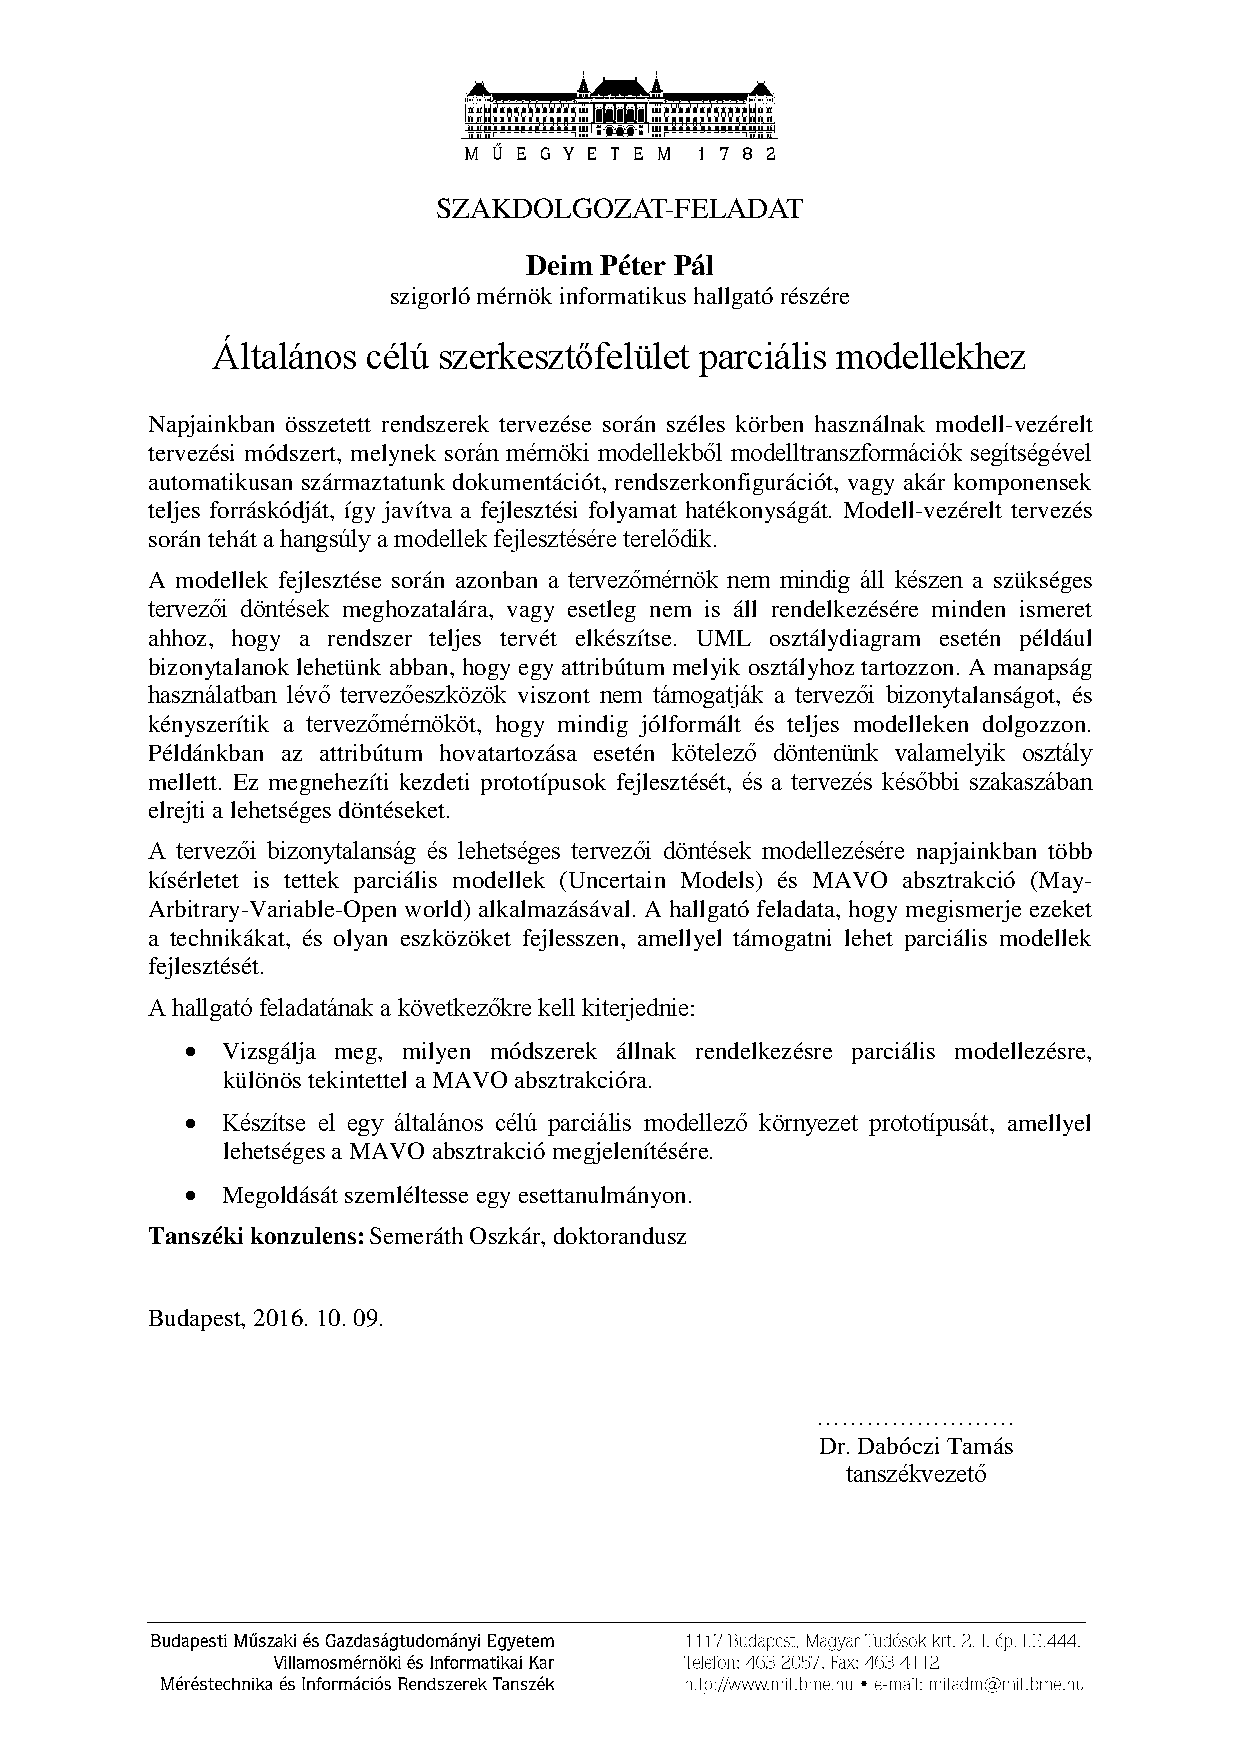
\includepdf[fitpaper=true, pages=-]{figures/feladat.pdf}
% Table of Contents
%~~~~~~~~~~~~~~~~~~~~~~~~~~~~~~~~~~~~~~~~~~~~~~~~~~~~~~~~~~~~~~~~~~~~~~~~~~~~~~~~~~~~~~
\tableofcontents\vfill


% Declaration and Abstract
%~~~~~~~~~~~~~~~~~~~~~~~~~~~~~~~~~~~~~~~~~~~~~~~~~~~~~~~~~~~~~~~~~~~~~~~~~~~~~~~~~~~~~~
\include{include/declaration} %TODO Hallgatói nyilatkozat -- TDK és OTDK esetén törlendő!
\pagenumbering{roman}
\setcounter{page}{1}

\selecthungarian

%----------------------------------------------------------------------------
% Abstract in Hungarian
%----------------------------------------------------------------------------
\chapter*{Kivonat}\addcontentsline{toc}{chapter}{Kivonat}

%Jelen dokumentum egy diplomaterv sablon, amely formai keretet ad a BME Villamosmérnöki és Informatikai Karán végző hallgatók által elkészítendő szakdolgozatnak és diplomatervnek. A sablon használata opcionális. Ez a sablon \LaTeX~alapú, a \emph{TeXLive} \TeX-implementációval és a PDF-\LaTeX~fordítóval működőképes.

Informatika világában manapság egyre elterjedtebb rendszerek és szoftverek fejlesztésénél, hogy modellező eszközöket használunk. Ezen eszközök hatékonyabbá teszik a tervezési munkálatokat, azonban többségük nem biztosít lehetőséget arra, hogy hiányos, vagy hibás modelleket készítsünk. 
\par
A szoftver általában már a tervezés alatt is megkövetelik azt, hogy a modellünk jólformált és teljes legyen. Ez sokszor olyan döntések meghozatalát kényszeríti ki, amivel nem szeretnénk a tervezés azon szakaszában foglalkozni. Ilyen esetben a legtöbb, amit tehetünk, hogy megjegyzéseket írunk fel. 
\par
Jó lenne egy olyan eszköz, ami a modellezés absztrakciós szintjén képes kezelni az ilyen döntéseket. 
Egyre többen foglalkoznak ezzel a kérdéssel, és sokféle megközelítés született már a problémára. Így került előtérbe a parciális modell és a MAVO (May-Arbitrary-Variable-Open word) absztrakció is. 
\par
Dolgozatomban egy olyan általános célú modellező környezetet mutatok be, aminek segítségével lehetséges részleges modelleket létrehozni és szerkeszteni. Az eszköz a MAVO absztrakciót támogatja. Ez úgy jelenik meg, hogy annotációkkal lehet felruházni a bizonytalan elemeket a modellben. Illetve egy esetben, az 'Open world' esetében magát a modellt lehet megjelölni. Az annotációk nem csupán jelzés értékűek, hanem funkcionalitás is társul hozzájuk. A modellező eszköz biztosít az annotációk feloldására automatizált megoldást, ezt finomításnak nevezik. Ezáltal csökkenthető a modell részlegessége, ami végül egy olyan modellhez vezethet, amiben egyáltalán nincsen annotáció, tehát teljes.
\par
Végeredményben, tehát a szerkesztővel minőségibb tervezés lehet megvalósítani, jobb dokumentálhatóságot biztosít és a prototípus gyártást is meggyorsítja.


\vfill
\selectenglish


%----------------------------------------------------------------------------
% Abstract in English
%----------------------------------------------------------------------------
\chapter*{Abstract}\addcontentsline{toc}{chapter}{Abstract}

%This document is a \LaTeX-based skeleton for BSc/MSc~theses of students at the Electrical Engineering and Informatics Faculty, Budapest University of Technology and Economics. The usage of this skeleton is optional. It has been tested with the \emph{TeXLive} \TeX~implementation, and it requires the PDF-\LaTeX~compiler.

In the world of IT it is increasingly popular these days to use modelling tools in the development of systems and softwares. These tools make the design more efficient but most of them are incapable of creating incomplete models. 
\par
Sofwares usually determine already at the design phase that the model is appropriately constructed and complete. This often leads to decisions that should not be necessary to deal with at this early stage of the designing process. The best we can do in such a case is to leave comments.
\par
A device that could handle this type of decisions on an abstract level of modelling would come handy. More and more professionals are busy with this problem and there are already several possible solutions from varous perspectives around. This is how the parcial model and the MAVO (May-Arbitrary-Variable-Open word) abstractions have come to the fore.
\par
In my thesis I will demonstrate a general modelling environment with the help of which it is possible to create and construct partial models. The tool supports the MAVO abstraction.  This works based on the possibility to assign annotations to uncertain elements in the model. And in the case of the 'Open world' the model itself can be assigned. The annotations are not only signs but they are also functional. The modelling tool provides an automated solution to unlock the annotations, which is called refinement. Thus the partiality of the model can be gradually reduced as far as it is complete and does not contain any annotations.
\par
In the end, it is possible to realize a quality design with the editor, which results in more precise documentation and speeds up the production.

\vfill
\selectthesislanguage

\newcounter{romanPage}
\setcounter{romanPage}{\value{page}}
\stepcounter{romanPage}    %TODO Összefoglaló -- TDK és OTDK esetén nem kötelező


% The main part of the thesis
%~~~~~~~~~~~~~~~~~~~~~~~~~~~~~~~~~~~~~~~~~~~~~~~~~~~~~~~~~~~~~~~~~~~~~~~~~~~~~~~~~~~~~~
\pagenumbering{arabic}

%TODO import your own content
%----------------------------------------------------------------------------
\chapter{\bevezetes}
%----------------------------------------------------------------------------

\section{Témamegjelölés}
Modell-vezérelt tervezésnek nagy szerepe van az informatikában egy szoftver vagy rendszer létrehozásánál. Modellek segítségével sokkal jobban, strukturáltabban és megbízhatóbban lehet tervezni. A modellek helyességét automatikusan ellenőrizni és a modellből kódot generálni is lehet. Ehhez a rengeteg eszköz áll rendelkezésünkre, viszont ezek nem mindenre nyújtanak megoldást. 
\section{Problémafelvetés}
Mai modellező eszközökkel általában nem lehetséges, hogy részleges, vagy hibás modelleket kezeljünk, elmentsünk. A modell készítése közben lehetnek döntések, amikkel nem is feltétlen szükséges foglalkozni az adott tervezési szakaszban, mégis ahhoz, hogy a modell érvényes legyen rákényszerül az ember. Ezeket az elemeket célszerű lenne valamilyen módon megjelölni és a szerkesztést folytatni. Előfordulhat hogy a modellben egy elem megléte, vagy a multiplicitása kétséges. Esetleg, olyan, hogy nem lehet eldönteni egy elemről hogy az melyik másikkal áll kapcsolatban.
\section{Célkitűzés}	
Dolgozatom célja, olyan általános célú modell elkészítése, aminek segítségével lehet részleges, vagy hiányos modelleket is ábrázolni. Például, előfordulhat olyan, hogy nem tudjuk eldönteni egy attribútumról, hogy melyik elemhez tartozik. Ilyet általában a modellező eszközök nem támogatnak. Célszerű lenne egy olyan általános módszert kitalálni, amivel lehetséges az ilyen és ehhez hasonló esetek megjelölése, kezelése.
\section{Kontribúció}
Kutatásom során megismerkedtem a részleges modellezés leglényegesebb aspektusaival. Létrehoztam egy olyan modellt, ami alapján lehetséges részleges modellek készítése. Ezután elkészítettem egy olyan vizuális szerkesztőfelületet, aminek a segítségével részleges modell példányokat lehet készíteni.  

\section{Hozzáadott érték}	
A Szerkesztő nem csupán egy megjelenítő eszközt biztosít a részleges modellnek, hanem más funkciókkal is ellátja azt. A modell finomítására is lehetőséget ad, ami a részleges modellek szerkesztésének egy fontos funkciója. Ennek jelentését és jelentőségét a dolgozat folyamán részletesen kifejtem.

\section{Dolgozat felépítése}
Előismeretek részben először egy konkrét példát mutatok  egy modellre. Későbbiekben ezen a példán keresztül mutatom be a részleges modellezés lényegét. A parciális modellezésnek először a szintaktikáját tárgyalom, majd a hozzá tartozó szemantikát ismertetem. Ezekben a részekben a részlegesség négy fajtáját emelem ki: May, Var, Abs, OW. Áttekintés a konkrét feladat tervét mutatom be egy ábra segítségével. Ismertetem a modell felépítését illetve a szerkesztőfelület lehetőségeit. Ezt követően a megvalósítási folyamat előzményeként kitérek a technológiákra, amikre szükség volt a megvalósításhoz.A szerkesztő minden eleméhez le van jegyezve annak megjelenése és működése. Végül a továbbfejlesztési lehetőségekről lesz szó. 

%\include{content/latex-tools}
%\include{content/thesis-format}
%\include{content/template-usage}
%----------------------------------------------------------------------------
\chapter{Előismeretek}
%----------------------------------------------------------------------------

%\section{Részleges modellek fajtái}
%\subsection{May}
%\subsection{Abs}
%\subsection{Var}
%\subsection{OW}
\section{Felvezetés}
%pl osztálydiagram

A részleges modellezést legegyszerűbben egy gyakorlati példán lehet bemutatni. Vegyük példának az UML \cite{UML} osztálydiagramját. Az UML (Unified Modeling Language) egy szabványos, objektumorientált modellezési nyelv, ami a tervezést, fejlesztést és egyéb folyamatokat segíti. Ezt a nyelvet informatikában és egyéb üzleti területeken egyaránt alkalmazzák. Magában foglal több diagram típust is.
\par
Az osztálydiagram egy strukturális diagram, segítségével egy rendszerben előforduló objektumokat, azok tulajdonságait és kapcsolatait lehet modellezni. Az objektumok téglalapokkal vannak jelezve, a hozzájuk tartozó attribútumok a téglalapon belül helyezkednek el és az elemek összekötésével a kapcsolatokat lehet jelezni.
\par
Az alábbi példában (lásd \autoref{jarmu}) egy járműnek az osztálydiagramja látható. A járműnek vannak attribútumai és tartalmaz ajtót, kereket és üléseket. Továbbá van neki egy meghajtása, ami egy absztrakt osztály. Ezek ugyan azon attribútumokkal van ellátva: id, típus, név. A meghajtásnak két leszármazottja van a benzinmotoros és a villanymotoros meghajtás. A benzinmotor tulajdonsága a hengerek száma a villanymotor tulajdonsága pedig az akkumulátor kapacitása.

\begin{figure}[!ht]
	\centering
	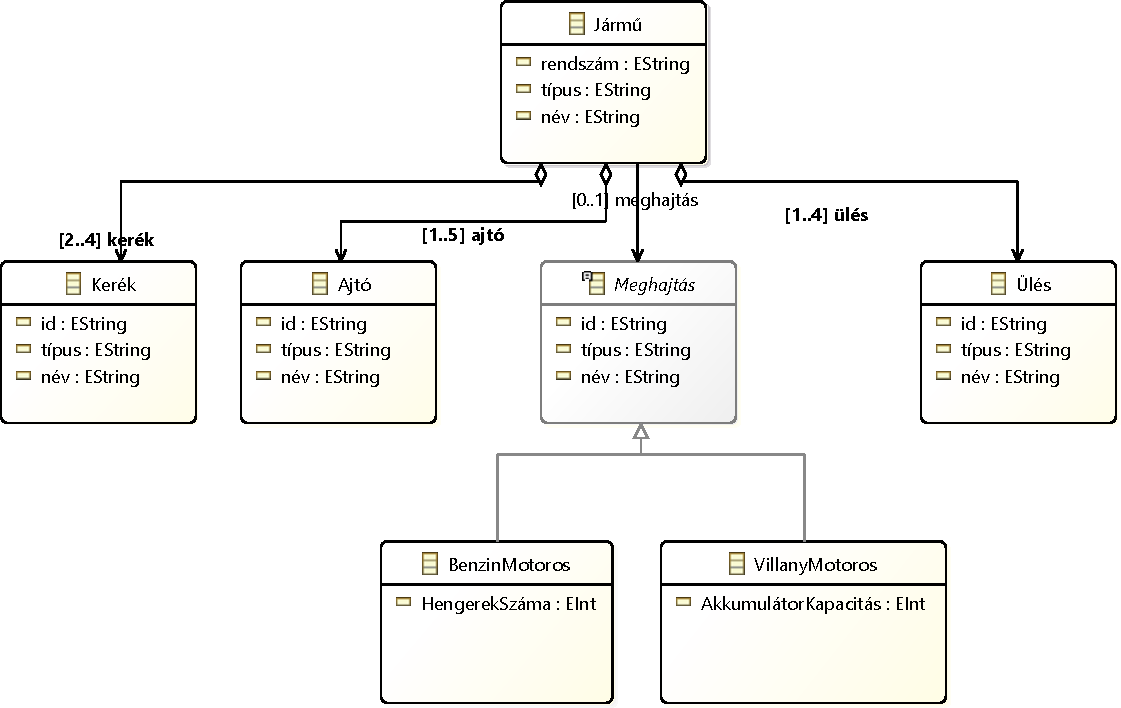
\includegraphics[width=130mm]{figures/vehicle.pdf}
	\caption{Jármű egyszerűsített osztálydiagramja} 
	\label{jarmu}
\end{figure}

\section{Részleges modell}
Részleges modell segítségével lehetőség van tervezői döntések dokumentálására. Általában a modellező eszközökkel csak érvényes modelleket lehet készíteni. Így a modell készítője belekényszerül olyan döntések meghozatalába, amiket csak később kéne meghozni. Emiatt elveszhetnek tervezői döntések. Részleges modellben lehetőség van ezeket a kétséges helyzeteket már a modellezés szintjén kezelni. Így a modell nem csupán strukturális információt tartalmaz, hanem a részlegességéről is, tehát hogy teljesen specifikált a modell vagy sem. Az előbbi példát tekintve, lehetséges az hogy a járműnek egyáltalán nem szeretnénk ajtót, mert például egy motort szeretnénk modellezni. Ekkor feleslegessé válik teljesen az ajtó jelenléte a modellben. Erről információt az UML szabályai szerint nem tudunk tárolni. Vagy feljegyezzük a lehetséges változtatást, vagy pedig létrehozunk egy másik diagramot, amibe van a járművön ajtó és egy olyat amiben nincs. Ezek egyike sem tűnik jó megoldásnak. Egy ilyen picike diagram esetén még akár átlátható de egy nagyobb, akár több száz elemből álló modell esetén, ha máshol is van ilyen kétség a végleges modellel kapcsolatban, akkor már kezelhetetlenné válik. Például 5 ilyen döntés esetében 2\^5 darab diagramot kéne párhuzamosan fejleszteni.
\par
Lehetőség van a modell finomítására is (lásd \autoref{finomit}). Finomítás során a parciális modellből kikerülnek bizonytalan elemek. Ez azt jelenti, hogy a modellben jelzett részlegesség mértéke csökkenthető és ennek eredményeképpen véges számú finomítás után a modellből teljesen eltűnnek a részlegességek.

\begin{figure}[!ht]
	\centering
	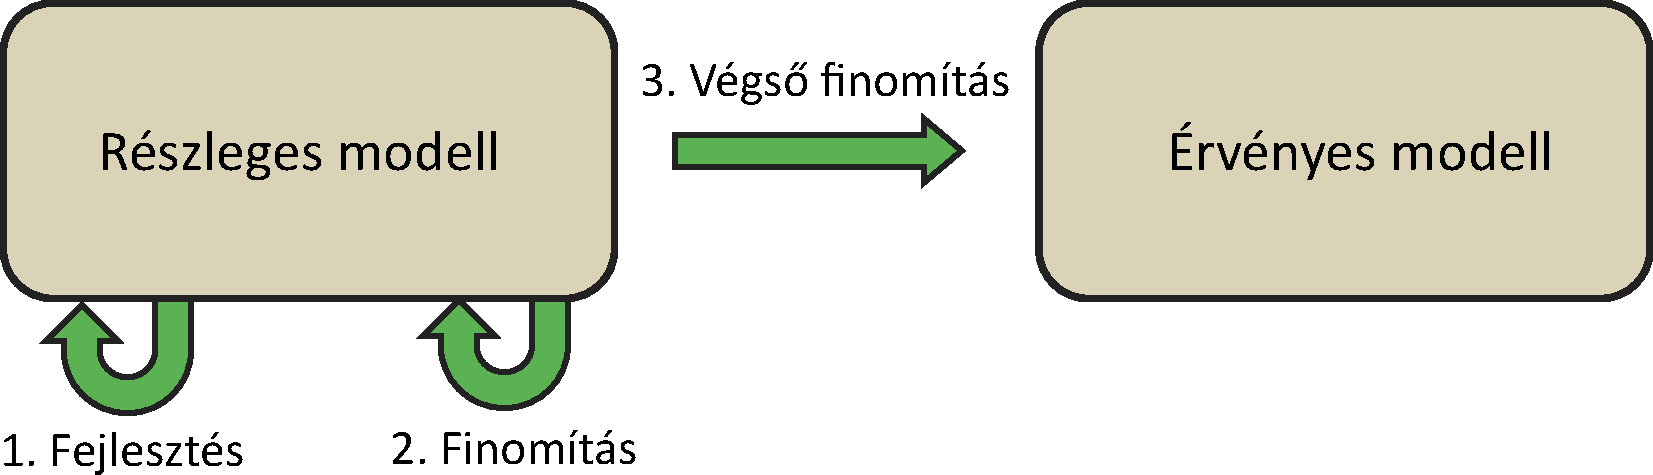
\includegraphics[width=130mm]{figures/finom.pdf}
	\caption{Finomítás menete} 
	\label{finomit}
\end{figure}

\subsection{Szintaktika}
Részleges modellek esetén annotációkkal lehet megjelölni a modellt, illetve annak elemeit. Modellezés során 4 fajta részlegességet jelölhetünk meg \cite{Salay}. Annotációk a modell minden elemére kerülhetnek, lehet attribútumra, objektumokra vagy akár élekre is.


\subsection{Szemantika}
\subsubsection{May}
Annotációkkal láthatjuk el a modellt, az alapján, hogy egy modellelem biztosan benne lesz a végleges modellben, vagy pedig még bizonytalan a léte. \textsf{’M’} May exist (lehet, hogy benne lesz a végleges modellben, de lehet, hogy nem), \textsf{’E’} Must exist (biztosan benne lesz a végleges modellben). A modell finomításával lépésről lépésre egyre kevesebb ’M’ lesz.  \textsf{’M’} az vagy átvált \textsf{’E’}–re, vagy teljesen kikerül a modellből. Akkor tekinthető a modell véglegesnek, ha már nem szerepel benne \textsf{’M’}-el megjelölt elem.
\par
Tegyük fel, hogy nem tudjuk milyen járművet akarunk még modellezni a kezdeti fázisban. Ezért a kiindulási objektummodellben elláttuk May annotációkkal a járműnek az ajtó elemét. Így finomítás során ez az elem később eltűnhet de akár meg is maradhat. Az a jármű aminek nincs ajtaja lehet akár egy motor, a két ajtós változat pedig egy autó. Erre példa az alábbi diagramrészlet (lásd \autoref{may}).

\begin{figure}[htp]
	\centering
	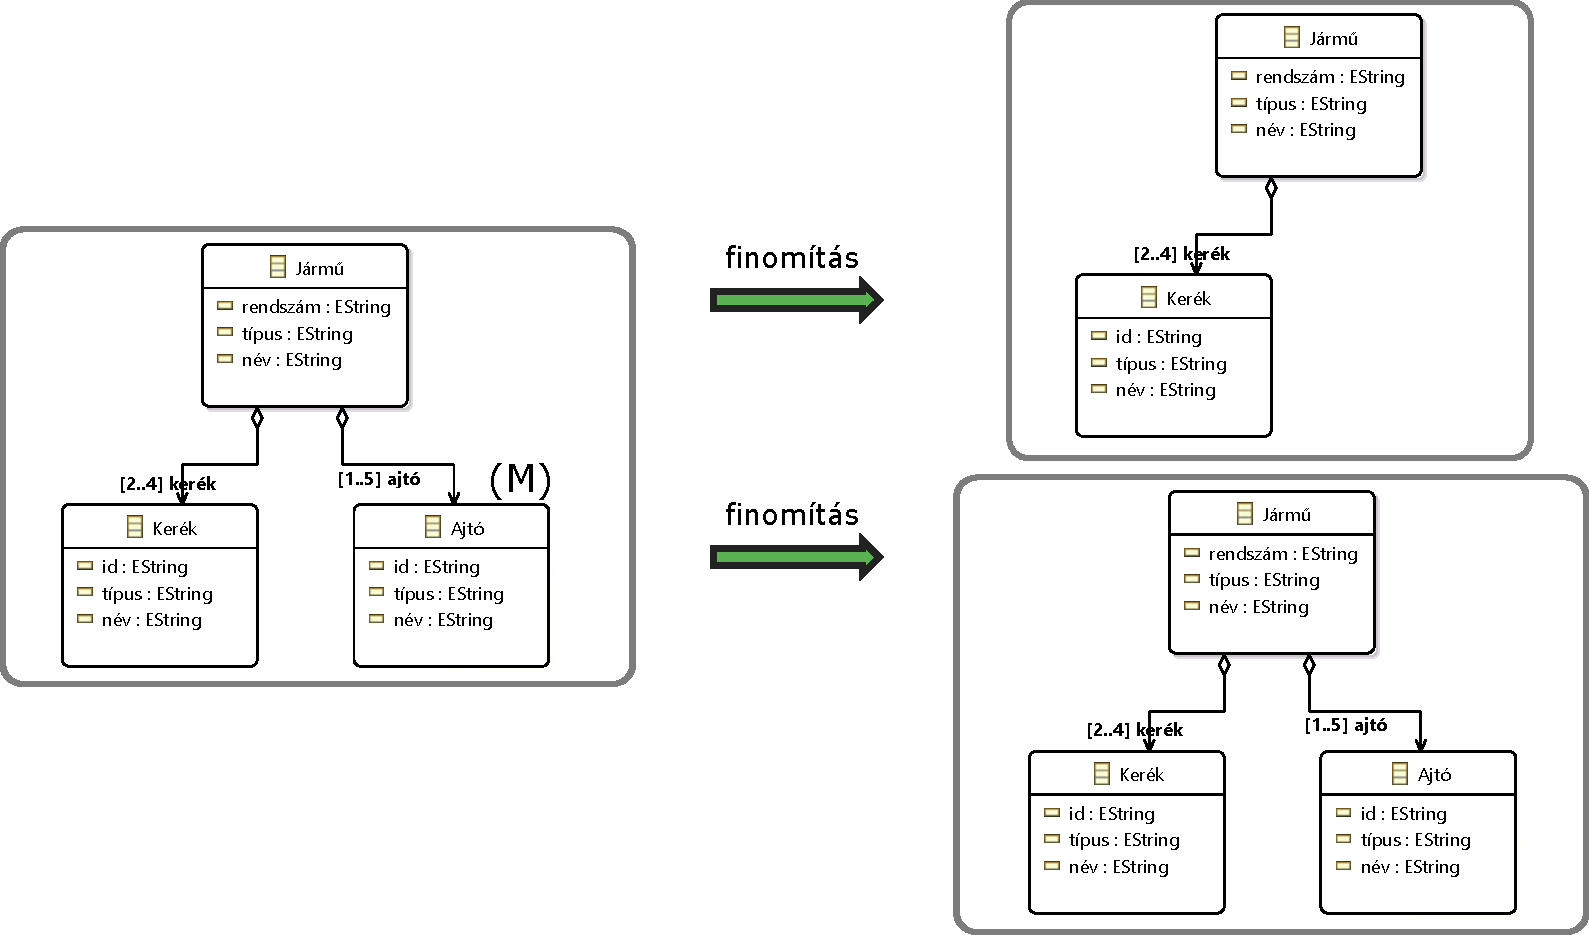
\includegraphics[width=130mm]{figures/may.pdf}
	\caption{May részlegesség feloldása} 
	\label{may}
\end{figure}

\subsubsection{Abs}
Ennek is két különböző annotálási módja lehet: \textsf{’P’}, Particular (egyedi elem) és \textsf{’S’}, azaz Set (egy vagy több elemet jelölhet). Particular az olyan elem, ami már biztosan benne lesz a végleges modellben, azonban a Set olyan elemet jelöl, ami lehet, hogy a végleges modellben több elemként fog megjelenni. Finomítások során az \textsf{’S’}-el megjelölt tagokat szétbontjuk több részre vagy meghagyhatjuk egyedi elemként, de a végleges modellben már csak egyedi elemek szerepelhetnek. 
%Legyen 'e' a modellnek egy eleme S(e) egy Set annotációval megjelölt elem. Finomítás után ez az elem 'n' darab elemre válhat szét, ahol \in
\par
Diagram kezdeti fázisában még nincs eldöntve, hogy az ülés az egyedi elem vagy sem, ezért meg van jelölve egy \textsf{’S’} annotációval. Finomítás során lehetséges, hogy az ülést megtartjuk eredeti formájában. A másik lehetőség viszont az, hogy szétbontjuk első illetve hátsó ülésre. Ebben az esetben ugyan azok a tulajdonságok lesznek meg mind a két ülésben de mégis modell szempontjából külön kezelendőek. Erre példa az alábbi diagramrészlet (lásd \autoref{abs}).

\begin{figure}[htp]
	\centering
	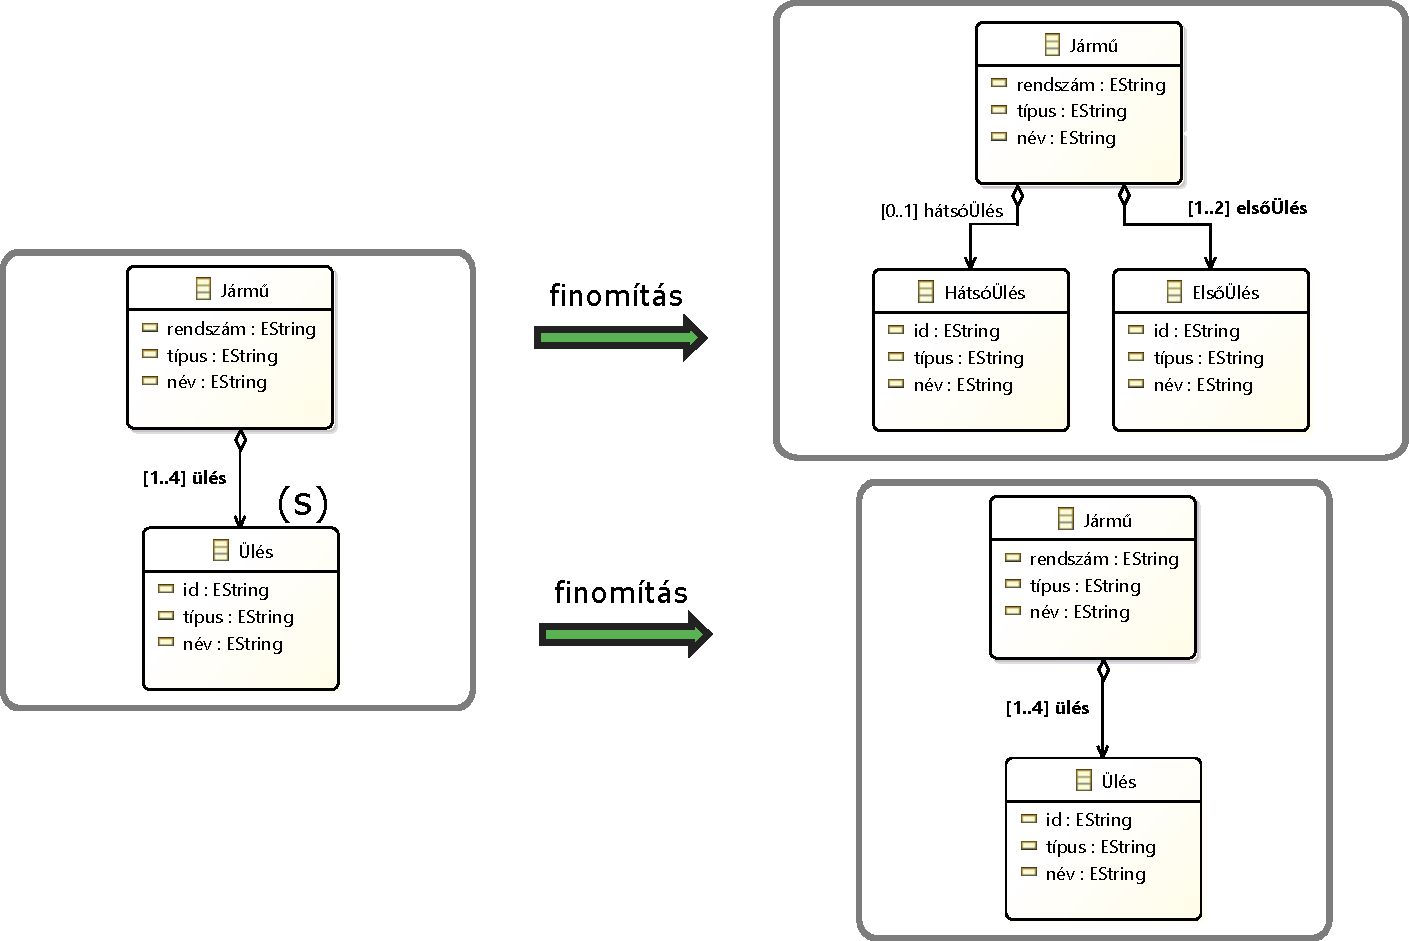
\includegraphics[width=130mm, keepaspectratio]{figures/abs.pdf}
	\caption{Abs részlegesség feloldása} 
	\label{abs}
\end{figure}

\subsubsection{Var}
Kétféleképpen lehet annotálni az elemeket: \textsf{’C’} Constant (konstans elem) és \textsf{’V’} Variable (változó elem). Bizonyos értelemben az Abs fordítottjának lehet tekinteni. Felveszünk több elemet, ami lehet, hogy későbbiekben összeolvasztunk egy elemmé, tehát fenn áll a lehetősége annak, hogy két elem megegyezik. Amikor elkezdünk egy modellt, akkor nem biztos, hogy meg tudjuk mondani elemekről, hogy azok a későbbiekben azonosak-e vagy különbözőek. A végleges modellben már csak konstans elemek lehetnek.
\par
Itt a példában (lásd \autoref{var}) látható, hogy a kezdeti állapotban még két külön kereke van a járműnek egyik kerekén kék dísztárcsa van a másik kereke pedig széles felnivel rendelkezik. Ezek meg lettek jelölve \textsf{'V'} annotációval. Finomítás után ez megmaradhat ilyen különálló formában, de akár összeolvaszthatjuk ezt a két kereket és a végeredményben egy kerék marad, ami mind a kettő kerék tulajdonságát magában hordozza.

\begin{figure}[htp]
	\centering
	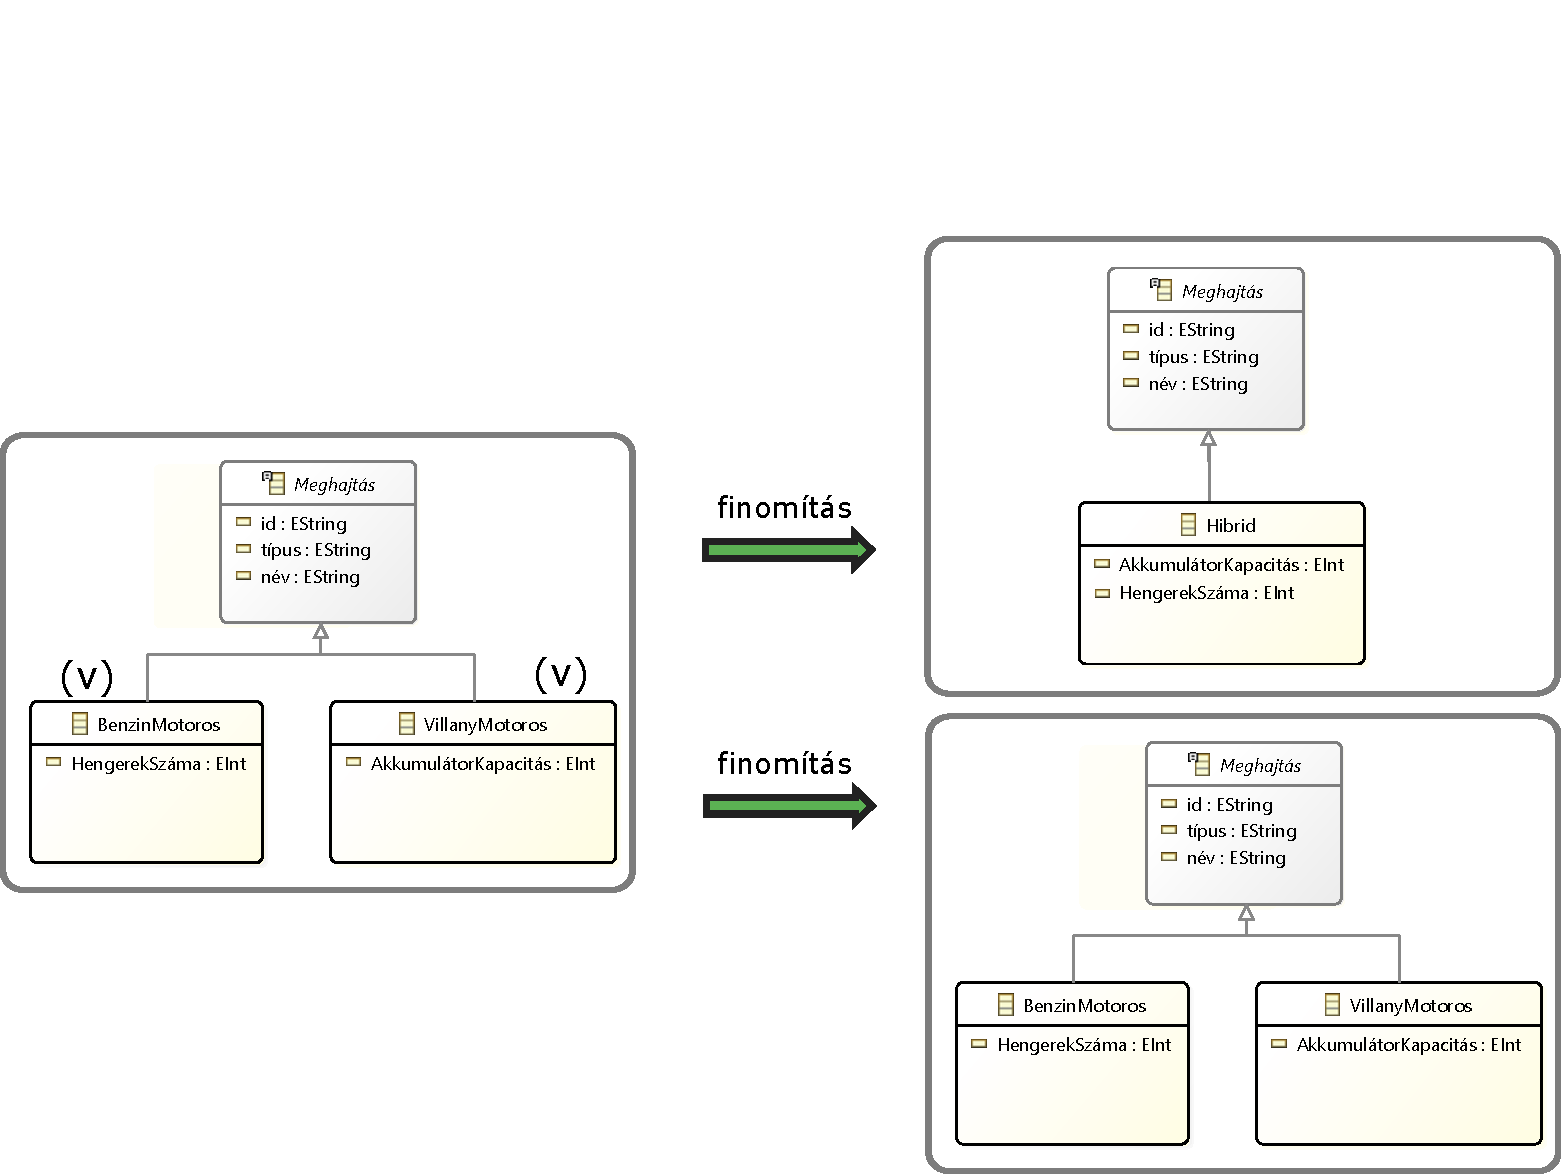
\includegraphics[width=130mm, keepaspectratio]{figures/var.pdf}
	\caption{Var részlegesség feloldása} 
	\label{var}
\end{figure}

\subsubsection{OW}
Modellezés folyamán lehet megjelölni azt, hogy a modell már végleges-e vagy sem, tehát adhatunk-e új elemeket a modellhez vagy nem. Ez a részlegesség nem a modell elemeire vonatkozik, hanem a teljes modellről árul el információt. 

%----------------------------------------------------------------------------
\chapter{Áttekintés}\label{chapter:overview}
%----------------------------------------------------------------------------
%Mit csinál
%Mire jó (szerkesztés, finomítás?, import? új objektumok...)
%(technológia nélkül)


Kutatásom során megnéztem egy másik modellezőeszközt, ami a 'May' részlegesség feloldására nyújt megoldást és ezzel kapcsolatos döntéstámogatást szolgáltat\cite{Michalis}. A többi részlegesség kezelését nem teszi lehetővé. célom egy olyan modellező eszköz elkészítése, ami segítségével lehetséges részleges modelleket készíteni. Ehhez olyan vizuális szerkesztőfelület társul, ami megkönnyíti ezt a folyamatot. Ahhoz, hogy ez generikusan működjön egy általános modell szükséges. Így ez a modell tartalmazni fog objektumokat, attribútumokat és az ezek közti kapcsolatot kifejező referenciákat. Ezen felül minden elemhez lehetséges rendelni \textit{May}, \textit{Var} vagy \textit{Abs} részlegességet. Magához a modellhez pedig \textit{OW} részlegességet lehet rendelni.
\par
A kapcsolódó editor képes részleges modellt létrehozni és manipulálni. Lehetőséget ad új objektumok, attribútumok, referenciák létrehozására. Ezen elemekhez a már fent említett részlegességek rendelhetők. A szerkesztő a részlegességek feloldására, tehát finomításra is biztosít eszközöket.(áttekintő ábra lásd \autoref{overview})



\begin{figure}[!ht]
	\centering
	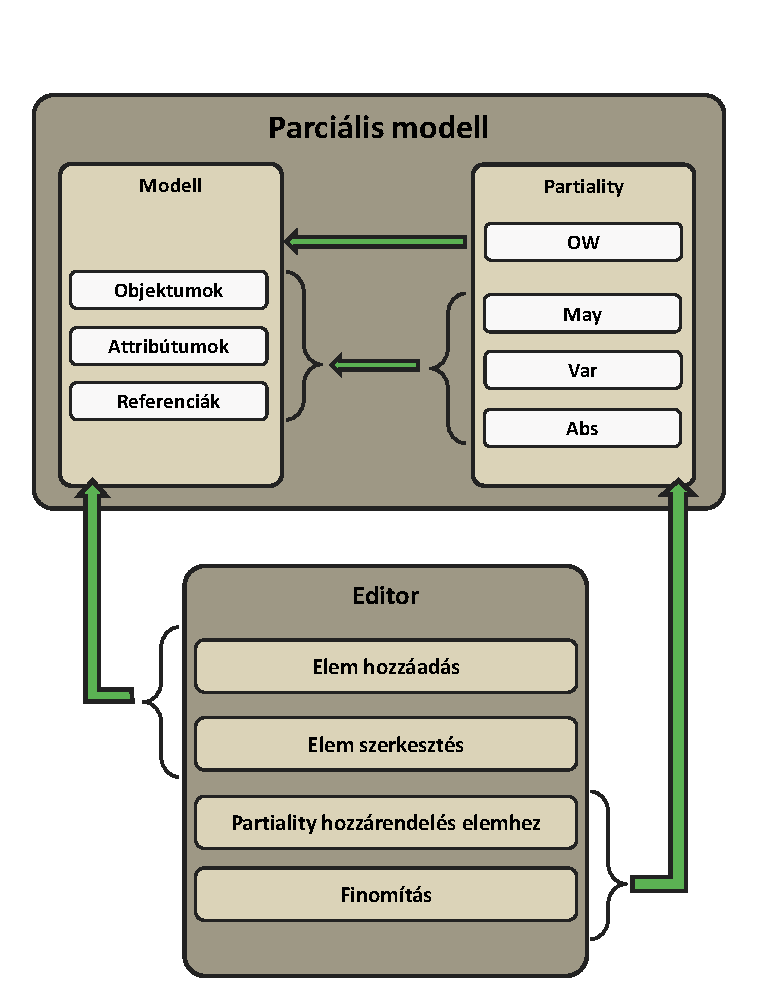
\includegraphics[width=100mm]{figures/overview.pdf}
	\caption{Részleges modell és a rajta végezhető műveletek} 
	\label{overview}
\end{figure}


%----------------------------------------------------------------------------
\chapter{Megvalósítás}\label{chapter:realization}
%----------------------------------------------------------------------------
\section{Felhasznált technológiák}
\subsection{Eclipse}
A feladatot Eclipse-be \cite{Eclipse} integrált tervezőeszközként valósítottam meg. Ez egy szabadon bővíthető nyílt forráskódú szoftverkeretrendszer. Sokféle modellező eszköz integrálható  Eclipse-be. Azért ezt választottam mert a modellezés általam használt részeihez is biztosít megfelelő keretrendszereket.
\subsection{Metamodell}
A metamodell összefoglalja egy modellezési nyelv legfőbb fogalmait, relációit és alapvető struktúráját. Egy olyan alapséma, amire illeszkedik az összes hozzá tartozó alacsonyabb absztrakciós szinttel rendelkező modell. 
Tegyük fel hogy M* modell M1 modellnek a metamodellje.
Akkor M* metamodell meghatározza az M1 modellben lévő elemeket, attribútumokat és ezeknek lehetséges kapcsolatait. Például az alábbi modelleknek (lásd \autoref{jarmupeldany}) a már korábban említett jármű modell tekinthető metamodelljének. Bal oldalon egy motor példánymodellje, jobb oldalon pedig egy biciklinek a modellje látható. Az általam elkészített metamodell a parciális modellek számára attól általános, hogy nem csupán az osztálydiagram metamodellje lehet, hanem ugyan úgy lehet a jármű metamodellje is. 

\begin{figure}[!ht]
	\centering
	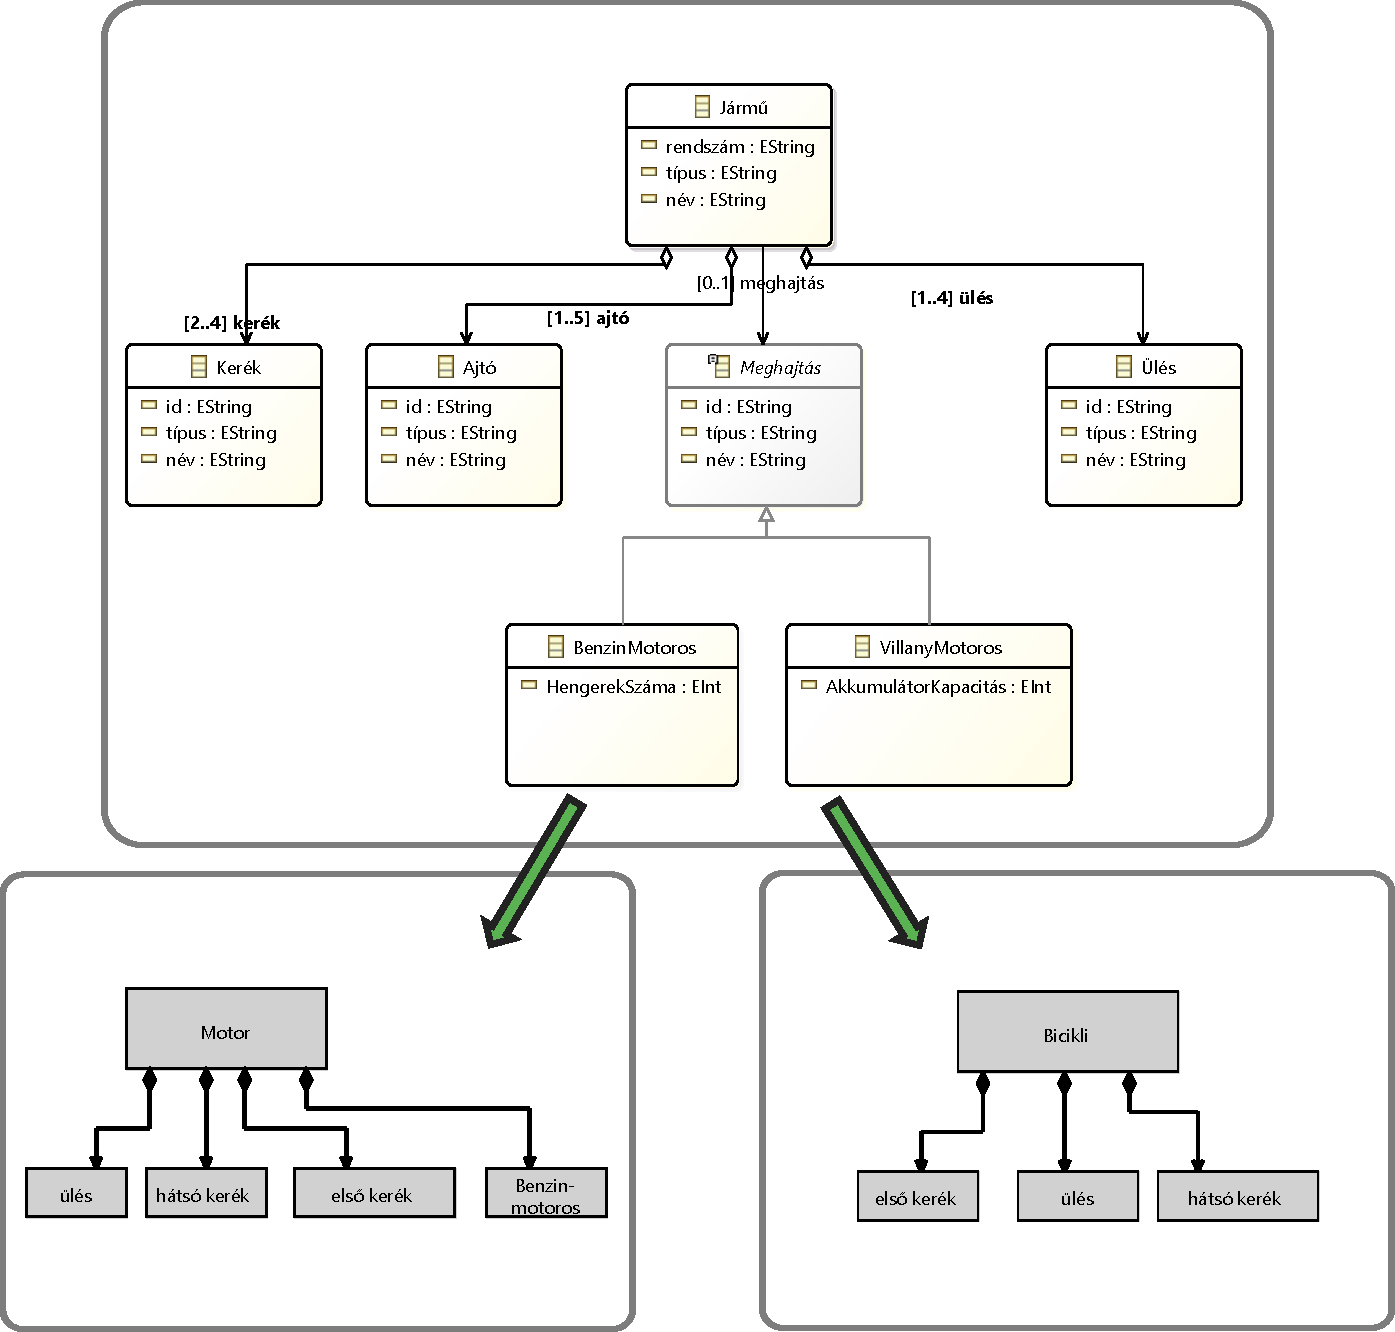
\includegraphics[width=110mm]{figures/meta.pdf}
	\caption{Jármű metamodellhez tartozó példánymodellek} 
	\label{jarmupeldany}
\end{figure}

\subsection{EMF}
\nocite{EMFtut}
EMF az Eclipse Modelling Framework \cite{EMF} rövidítése. Ez egy olyan keretrendszer, mely modellek készítését teszi lehetővé. Az Eclispe-be beépülő EMF modellező eszközök segítségével könnyedén lehet grafikusan metamodelleket alkotni, melyből később konkrét példánymodellt készíthetünk. Továbbá lehetőséget biztosít metamodellből java kódot generálni, ami leképezi a modell elemeit osztályokba és a hozzá tartozó kapcsolatokat és attribútumokat is.

\subsection{Sirius}
\nocite{SiruisTutNagyASz}
\nocite{SiruisTutStart}
\nocite{SiruisTutAdv}
Ez egy szintén Eclipse-be épülő keretrendszer \cite{Sirius}. Ez lehetővé teszi hogy EMF modellekhez vizuális megjelenítő és szerkesztő felületet készítsünk. Lehetőség van új objektumok létrehozására, törlésére és szerkesztésére. Az egyes elemek módosítását megszorításokhoz lehet kötni. A szerkesztő elkészítéséhez egy "viewpoint specification" projektet kell létrehozni, majd ezen belül egy "odesign" kiterjesztésű fájlt. A fájl definiálja a szerkesztő működését, amiben a következőket műveletek végezhetők:
\begin{itemize}  
	\item Be lehet állítani milyen modellt kezeljen.
	\item Reprezentáció típusa is megadható. Például: diagram, táblázat, fastruktúra.
	\item Modellelemek stílusa, megjelenése. Például: szín, forma.
	\item Mi történjen egy elem módosításánál, törlésénél, vagy létrehozásánál.
	\item Lehet külső java kódot futtatni benne.
	\item Az egyes funkciók működését Aql kifejezésekkel lehet leírni. Aql az Annotation Query Language \cite{Aql} rövidítése. Lambda \cite{Lambda} kifejezésekhez hasonlóan lehet alkalmazni. 
	
\end{itemize}


%Ebben a fájlban be kell állítani milyen modellel szeretnénk dolgozni és azután lehet a modellhez tartozó editor működését és megjelenését definiálni. Ki lehet választani milyen típusú reprezentációt szeretnék a modellemnek, például: diagram, táblázat, fastruktúra. Meg lehet adni hogy a modellben lévő elemek vizuálisan hogyan jelenjenek meg. Ez a stílus akár dinamikusan változhat az elem tulajdonságától függően. Ebben a fájlban lehet pontosan megadni, hogy mi történjen egy elem létrehozásánál, törlésénél vagy módosításánál. Ezen események bekövetkezése kiválthatnak további eseményeket, ezáltal láncba fűzhetők. Például kitörlök egy elemet és ennek következtében módosítok egy másikat. A Sirius-szal lehet elágazásokat definiálni (switch-case, if) és iterációt is támogat (for ciklus). Sirius képes külső Java kód futtatására, amivel bővíthető a szerkesztőfelület funkcionalitása.

%\subsection{Aql}
\nocite{Acceleo}
\nocite{OCL}
%Az Annotation Query Language \cite{Aql} rövidítése. Lambda \cite{Lambda} kifejezésekhez hasonlóan lehet alkalmazni. 
%A lambda kifejezés egy névtelen függvény, ami 
%Az editor elkészítésében van nagy szerepe. Az egyes funkciókat előfeltételeit lehet leírni ezen a nyelven. 

%\section{Metamodell szerkezete}

\section{Általános modell}

Egy általános modell elemekből áll, amik tulajdonságokkal rendelkeznek, az elemek között pedig kapcsolatok vannak. Tehát olyan meta modellt kell készíteni, ami mindezeket magába foglalja. A metamodell elkészítéséhez EMF-et használtam (lásd \autoref{model}).

\begin{figure}[!ht]
	\centering
	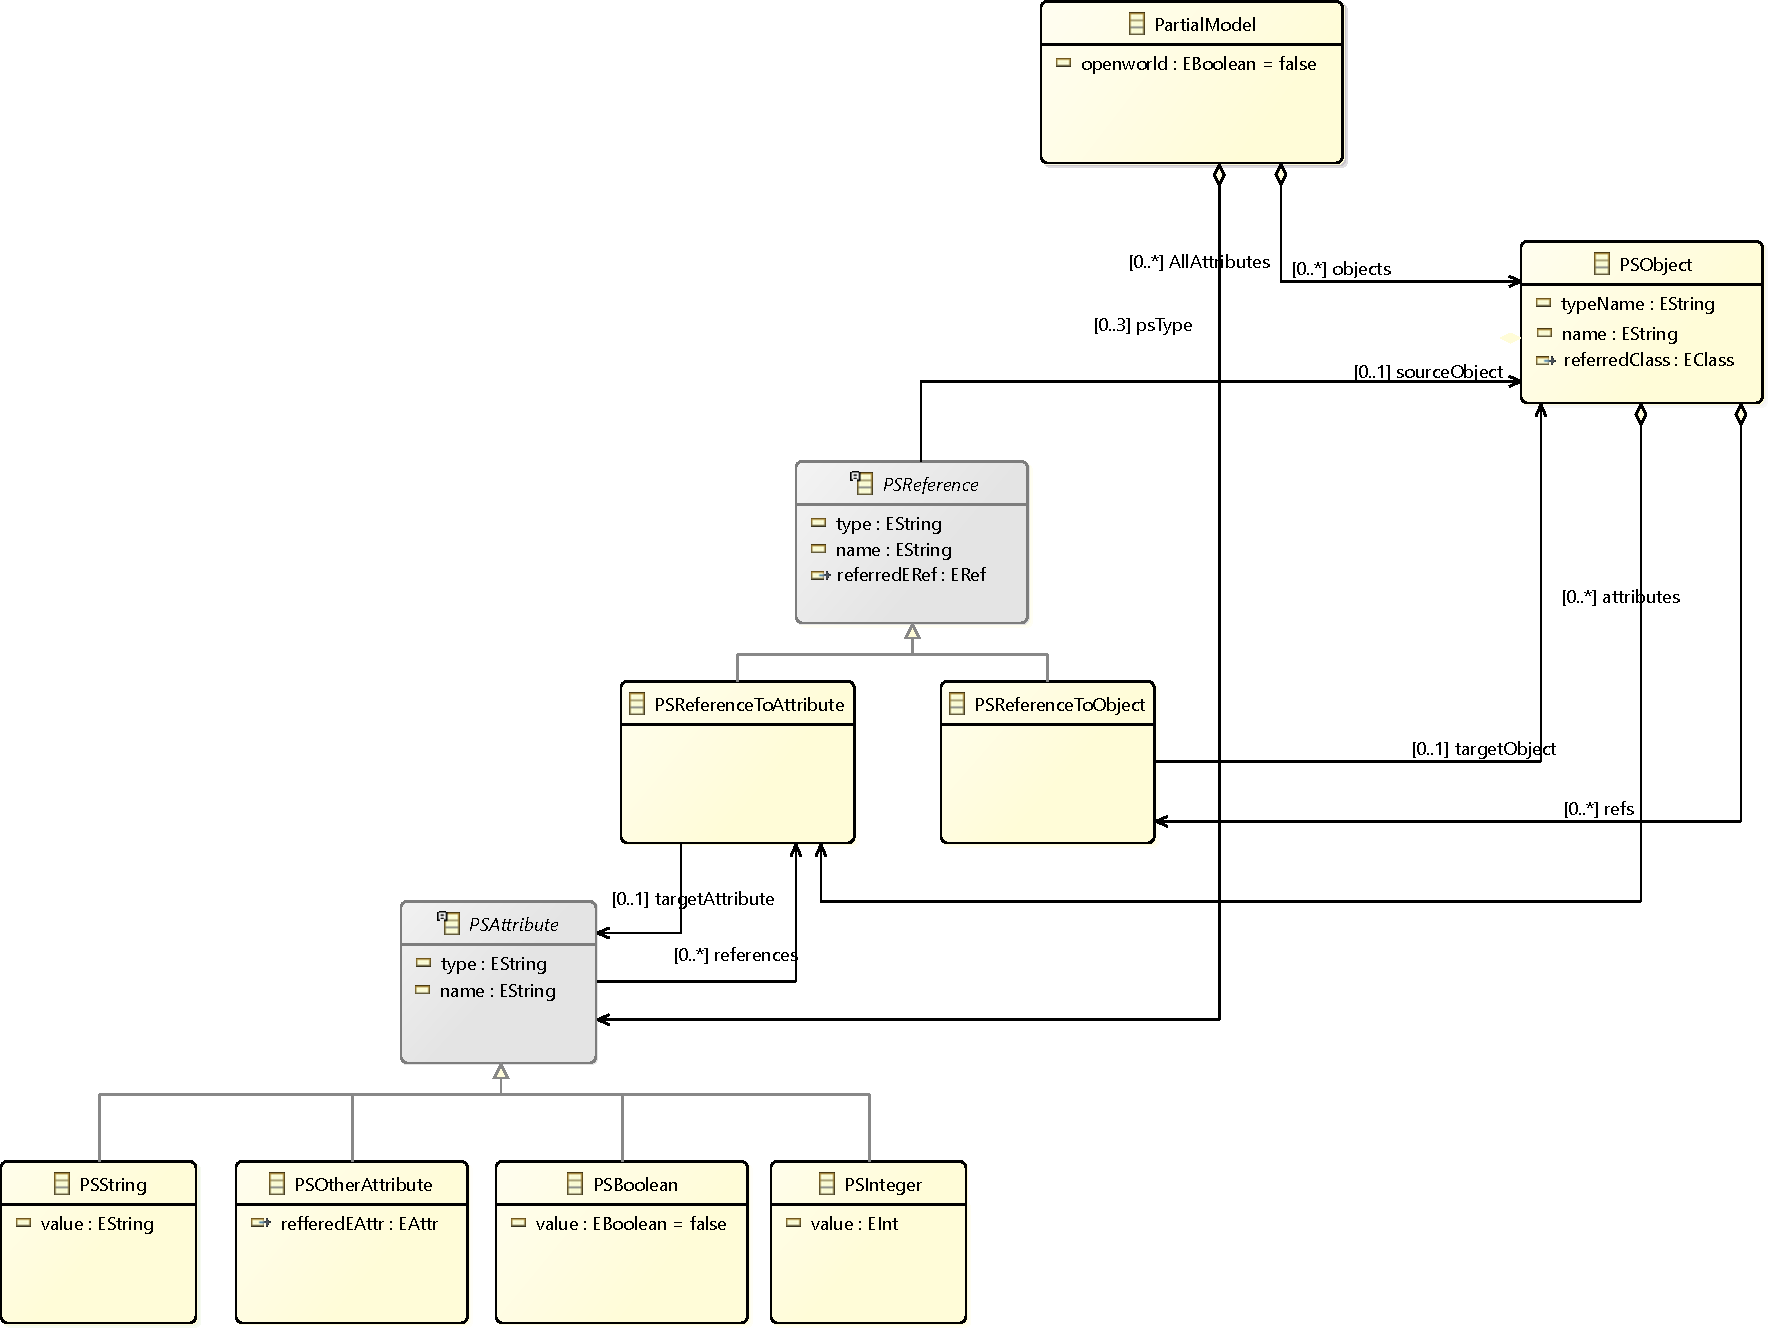
\includegraphics[width=150mm]{figures/partialmodel01.pdf}
	\caption{Általános modell, ami legtöbb modell metamodelljének tekinthető} 
	\label{model}
\end{figure}

\subsection{Objektum (PSObject)}
A modellben a PSObject-ek reprezentálják az általános modell elemeit. Rendelkezik névvel (name), ami egy 'EString' és referált osztállyal (ReferredEClass) aminek típusa 'EClass'. a referált osztály mutatja meg, hogy az objektum milyen típusú. %A PSObject-hez lehet részlegességeket rendelni, ennek a neve PSType. így a PSObject-en keresztül tudunk részlegességet rendelni a hivatkozott objektumhoz, ami erre egyébként nem lenne képes. 
PSObjectek tartalmaznak tetszőleges mennyiségű referenciát másik objektumokra (PSReferenceToObject) és attribútumokra (PSReferenceToAttribute).

\subsection{Referencia (PSReference)}
 Az elemek közötti kapcsolatokat reprezentálják. Fontos, hogy ezek is külön elemként jelenjenek meg a modellben, hisz ehhez is szeretnénk majd részlegességet társítani annotációk formájában. A PSReference egy absztrakt objektum két leszármazottja van a  PSReferenceToAttribute és PSReferenceToObject. Erre azért volt szükség mert logikailag kifejezi azt, hogy az attribútum valamelyik objektum része és csak azzal együtt érvényes, míg egy objektum önmagában is értelmezhető. Rendelkezik névvel (name) és egy 'ERefference' típusú attribútummal (ReferredERef). 'ReferredERef' segítségével adható meg a referencia típusa. Van neki forrásobjektuma (sourceObject) és célobjektuma (targetObject) vagy célattribútuma (targetAttribute).

\subsection{Attribútum (PSAttribute)}
Az objektumok tulajdonságai külön egy PSAttribute nevű elemben vannak hozzárendelve az objektumokhoz, így lehetőség van az attribútumokhoz is részlegességet rendelni. Lehetséges továbbá az is hogy egy attribútum több objektumhoz is tartozzon, ugyanis az attribútumokat nem közvetlenül a PSObjeckt-ek tárolják hanem csak hivatkoznak rájuk. Azonban az attribútumok tárolják a rájuk mutató PSReference-ek referenciáit. PSAttribute absztrakt ezért több fajtája lehet.

\begin{itemize}  
	\item PSString: 'String' típusú attribútumot reprezentál. Értéke 'String' típusú lehet csak.
	\item PSBoolean: 'Boolean' típusú attribútumot reprezentál. Értéke kizárólag 'Boolean' lehet.
	\item PSInteger: 'Integer' típusú attribútumot reprezentál. Értéke csak 'Int' típusú lehet.
	\item PSOtherAttribute : Tartalmaz egy 'EAttribute'-ra mutató referenciát. (refferedEAttribute). Tetszőleges egyéb attribútumot referálhat.
\end{itemize}


\section{Kiegészítés részleges modellé}

\subsection{OW részlegesség}
Az \textit{OW} részlegességet a modell gyökerében egy boolean változóval tudjuk szemléltetni.

\subsection{Részlegesség típusa (PSType)}
Minden egyes modellbeli elemhez tudnunk kell társítani annotációkat. Ezt a PSType-al tehetjük meg (lásd \autoref{partialmodel}). Ilyen PSType elemet tartalmazhat az attribútum a referencia és az objektum is. Egy időben több fajta részlegesség is lehet egy elemen. Részlegességek szerint három leszármazottja van a PSType-nak:

\begin{itemize}  
	\item MayType: \textit{May} részlegességet jelöl, azon az elemen amelyik tartalmazza. 
	\item AbsType: \textit{Abs} részlegességet jelöl, azon az elemen amelyik tartalmazza.
	\item VarType: \textit{Var} részlegességet jelöl, azon az elemen amelyik tartalmazza.
\end{itemize}

\begin{figure}[!ht]
	\centering
	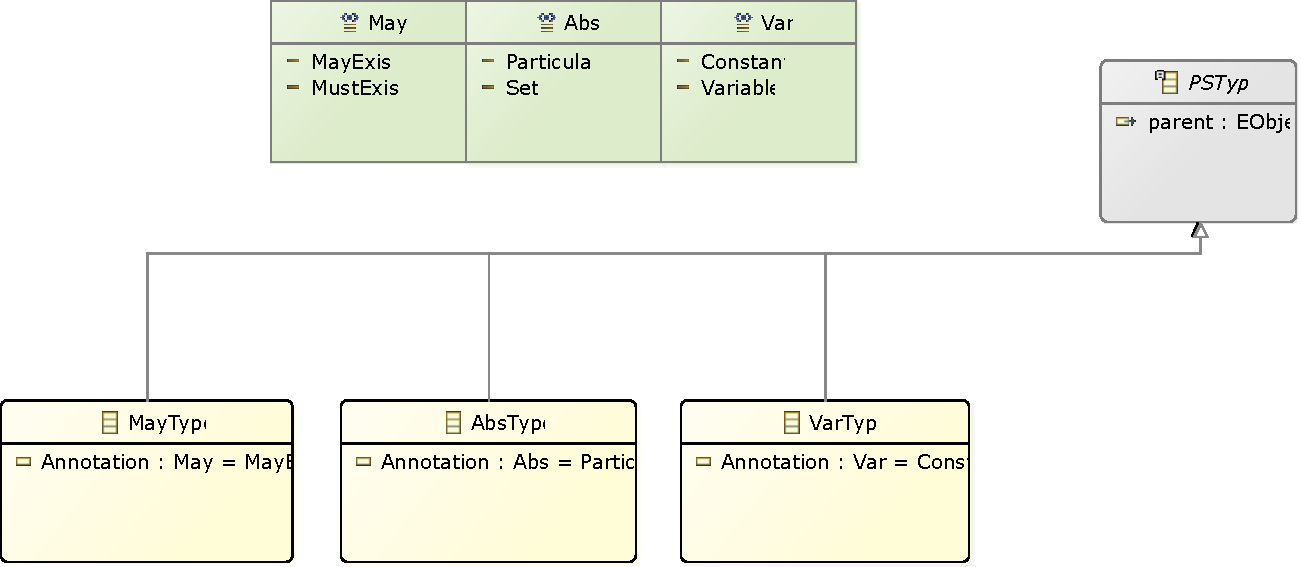
\includegraphics[width=150mm]{figures/partialmodel02.pdf}
	\caption{Általános modell kiegészítve részleges modellekre jellemző tulajdonságokkal}
	\label{partialmodel} 
\end{figure}

\section{Szerkesztőfelülete}
\subsection{Modell elemeinek stílusa és alapfunkciók}
\subsubsection{Objektum (PSObject)}
Világoszöld téglalapként jelenik meg (lásd \autoref{obj}).  A téglalap fejrészében megjelenik az objektum neve.
\begin{figure}[!ht]
	\centering
	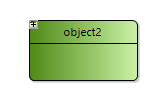
\includegraphics{figures/obj.PNG}
	\caption{PSObject}
	\label{obj} 
\end{figure}
\\\\
Funkciók:
\begin{itemize}  	
	\item Bal felső sarkában pedig egy kis '+' jel segítségével megjeleníthetjük a hozzá tartozó attribútumokat. Amennyiben ezek láthatóak akkor egy '-' jel jelenik meg amivel elrejthetjük. 	
	
	\item PSObject létrehozása az eszköztárból kiválasztva lehetséges, majd a szerkesztőfelületre kattintva megjelenik egy négyzet egy alapértelmezett névvel. A név formátuma: 'Object\{szám\}'. A szám helyén egy automatikusan generált szám kerül, a már meglévő PSObject-ek száma növelve eggyel.

	\item Az objektum nevére rákattintva az közvetlenül szerkeszthetővé válik. A többi tulajdonság a Sirius által alapból biztosított 'Properties' fülön érhető el. 
	
	\item Törlés esetén megsemmisül az objektumból kivezető összes referencia. Sirius tartalmazás esetén automatikusan kitörli az objektumban lévő egyéb elemeket. Az objektumra mutató referenciák viszont nem törlődnek maguktól, mert a forrás PSObject-ben vannak. Mivel a PSObject nem tárolja a rá mutató éleket így először az összes PSObject referenciáján végigiterálva kitörli azokat, amik rá mutatnak, majd törli önmagát is. 
\end{itemize}


\subsubsection{Referencia (PSReference)}
A felületen szürke vonalként jelenik meg. Összeköthet PSObject-et attribútummal vagy egy másik PSObject-el. Utóbbi esetben a vonal végén nyíl is van. A referencián szövegesen megjelenik neve és zárójelben a hozzá tartozó részlegességek is. Amennyiben rákattintunk a referencia vonalára kétszer, akkor egy új ablak jelenik meg. Ebben az ablakban egy narancssárga négyzeten a referencia neve van. Ez azért fontos mert itt tudunk hozzáadni részlegességeket a referenciához a későbbiekben (lásd \autoref{ref}).
\begin{figure}[!ht]
	\centering
	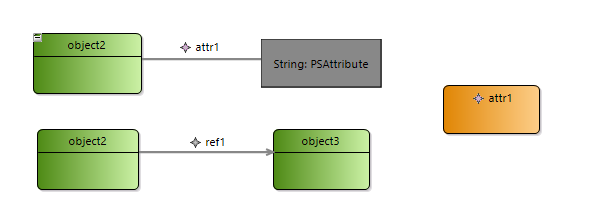
\includegraphics{figures/ref.PNG}
	\caption{PSReference (baloldalt a részleges modellen megjelenő formában vonalként, jobb oldalon a rákattintás utáni nézet látható)}
	\label{ref} 
\end{figure}
\\\\
Funkciók:
\begin{itemize}  	
	\item Kétszer rákattintva egy referenciára megjelenik egy új szerkesztőfelület. Itt csak egy narancssárga téglalap van a referencia nevével. Erre a nézetre azért van szükség, mert részlegességek így könnyebben kezelhetők. A részlegességek magyarázatánál bővebben lesz erről szó.
	
	\item Létrehozása a szerkesztőfelület oldalán lévő sávból kiválasztva lehetséges (reference). Aztán egy PSObject-re kattintva a kezdőpontja, majd második kattintásra a cél objektuma vagy attribútuma jelölhető ki a referenciának. A kiválasztó felületen nincs külön referencia objektumra és attribútumra, ez a felhasználó számára rejtve marad, azonban a háttérben mégis külön kezelődik. Referencia létrehozásának a logikájában van egy elágazás (switch), ami vizsgálja, hogy a célobjektum, tehát amire másodjára kattintunk az milyen típusú. A referencia típusát aql kifejezéssel lehet eldönteni. A referencia nevét hasonlóan a PSObject-hez aql segítségével generálja: 'attr\{szám\}' vagy 'ref\{szám\}'. Itt a 'szám' a forrás objektumból kiinduló attribútumokra vagy objektumokra mutató referenciák számát veszi figyelembe. Attribútumra mutató referencia esetében kicsit különbözik a működés. Amennyiben a referált attribútumra már mutat másik referencia, akkor az új referenciához automatikusan hozzá generálunk egy May részlegességet. Ennek az az értelme, hogy gyakorlatban nem fordulhat elő olyan, hogy egy attribútum több objektumhoz is tartozik.
	
	\item Éleket át lehet huzalozni, azaz másik célelemet lehet választani nekik. PSObject-re mutató élt nem lehet megváltoztatni PSAttribute-ra mutató élre és fordítva se. Új cél kiválasztása esetén a régi felülíródik. Attribútum esetében a régi attribútumból törlődik az él referenciája és az új attribútumba íródik be. Ha attribútumról olyan attribútumra húzzuk át az élet, amibe már vezet él akkor ahhoz  automatikusan hozzá generálódik egy 'May' részlegesség, mint ahogy az új él létrehozásnál is történt.
	
	\item Törlés esetén az objektum és a hozzá tartozó referenciák törlődnek.
\end{itemize}

%\begin{figure}[!htp]
%	\centering
%	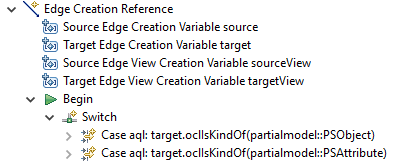
\includegraphics[width=100mm]{figures/refcreation.PNG}
%	\caption{Referencia létrehozásának logikája}
%	\label{refcreation} 
%\end{figure}

\subsubsection{Attribútum (PSAttribute)}
Szürke téglalapként jelenik meg a szerkesztőfelületen (lásd \autoref{attr}). Az attribútum típusa és értéke a téglalap közepén látható kettősponttal elválasztva.
\begin{figure}[!ht]
	\centering
	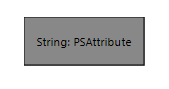
\includegraphics{figures/attr.PNG}
	\caption{PSAttribute}
	\label{attr} 
\end{figure}
\\\\
Funkciók:
\begin{itemize}  	
	\item Létrehozása az eszköztárról kiválasztva lehetséges, ezután a szerkesztő panelen kattintva létrejön egy attribútum. Ez nem tartozik még egyetlen objektumhoz sem.
	
	\item A típusának és értékének szerkesztése lehetséges a Sirius által biztosított 'Properties' fülön.
	
	\item Törlésénél végig iterál az összes rá mutató referencián és kitörli azokat, majd törli önmagát is.	

\end{itemize}

\subsubsection{Részlegesség típusa (PSType)}
A szerkesztőfelületen világoszöld téglalapként jelenik meg az elem mellett, amihez hozzá lett rendelve (lásd \autoref{part}). Referencia esetén zárójelben látszik az él neve előtt, de ha kétszer rákattintunk a referenciára, hogy megnyissuk a szerkesztőfelületét, ott az élet reprezentáló narancssárga téglalap mellett fog megjelenni (lásd \autoref{obj}).
\begin{figure}[!ht]
	\centering
	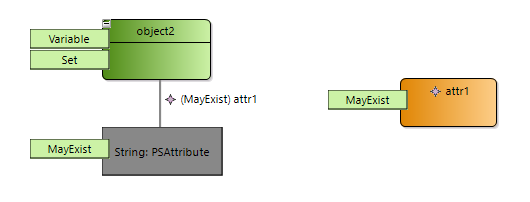
\includegraphics{figures/part.png}
	\caption{PSType (baloldalt a részleges modell szerkesztőfelülete, jobb oldalon a referencia szerkesztőfelülete)}
	\label{part} 
\end{figure}
\\\\
Általános funkciók:
\begin{itemize}  	
	\item Létrehozása a szerkesztőfelület oldalán lévő sávból kiválasztva lehetséges (May, Abs, Var), utána arra az elemre kattintva amelyikhez a részlegességet hozzá akarom rendelni létrejön a PSType. Él esetében ugyan ez a referencia saját szerkesztőfelületén lehetséges.
	
	\item Törlés esetén eltávolítja magát az objektumból.
\end{itemize}

\subsection{Finomítás funkció}
Duplán kattintva a PSType-ra történik meg a feloldása a részlegességnek. A PSType-nak három fajtája van, amik különböző módokon viselkednek attól függően, hogy milyen típusú elemre vannak rátéve, ezért ezeket külön tárgyalom. 

\subsubsection{PSObject-May részlegesség feloldása}
Feloldásnál az objektum kitörli a belőle kivezető éleket, majd az összes más objektumból rá mutató élet. Kitörli az attribútumra mutató éleket is és amennyiben az adott attribútumra nem vezet más objektumból él akkor az is törlődik (lásd \autoref{objmay}). Ezután maga az objektum is törlődik.
%Aql feltétel, ami azt vizsgálja, hogy nem vezet-e más objektumból él az attribútumba:
%\begin{align}
% aql:ref.targetAttribute.references->forAll(x | x.sourceObject = element.eContainer())
%\end{align}
\begin{figure}[!ht]
	\centering
	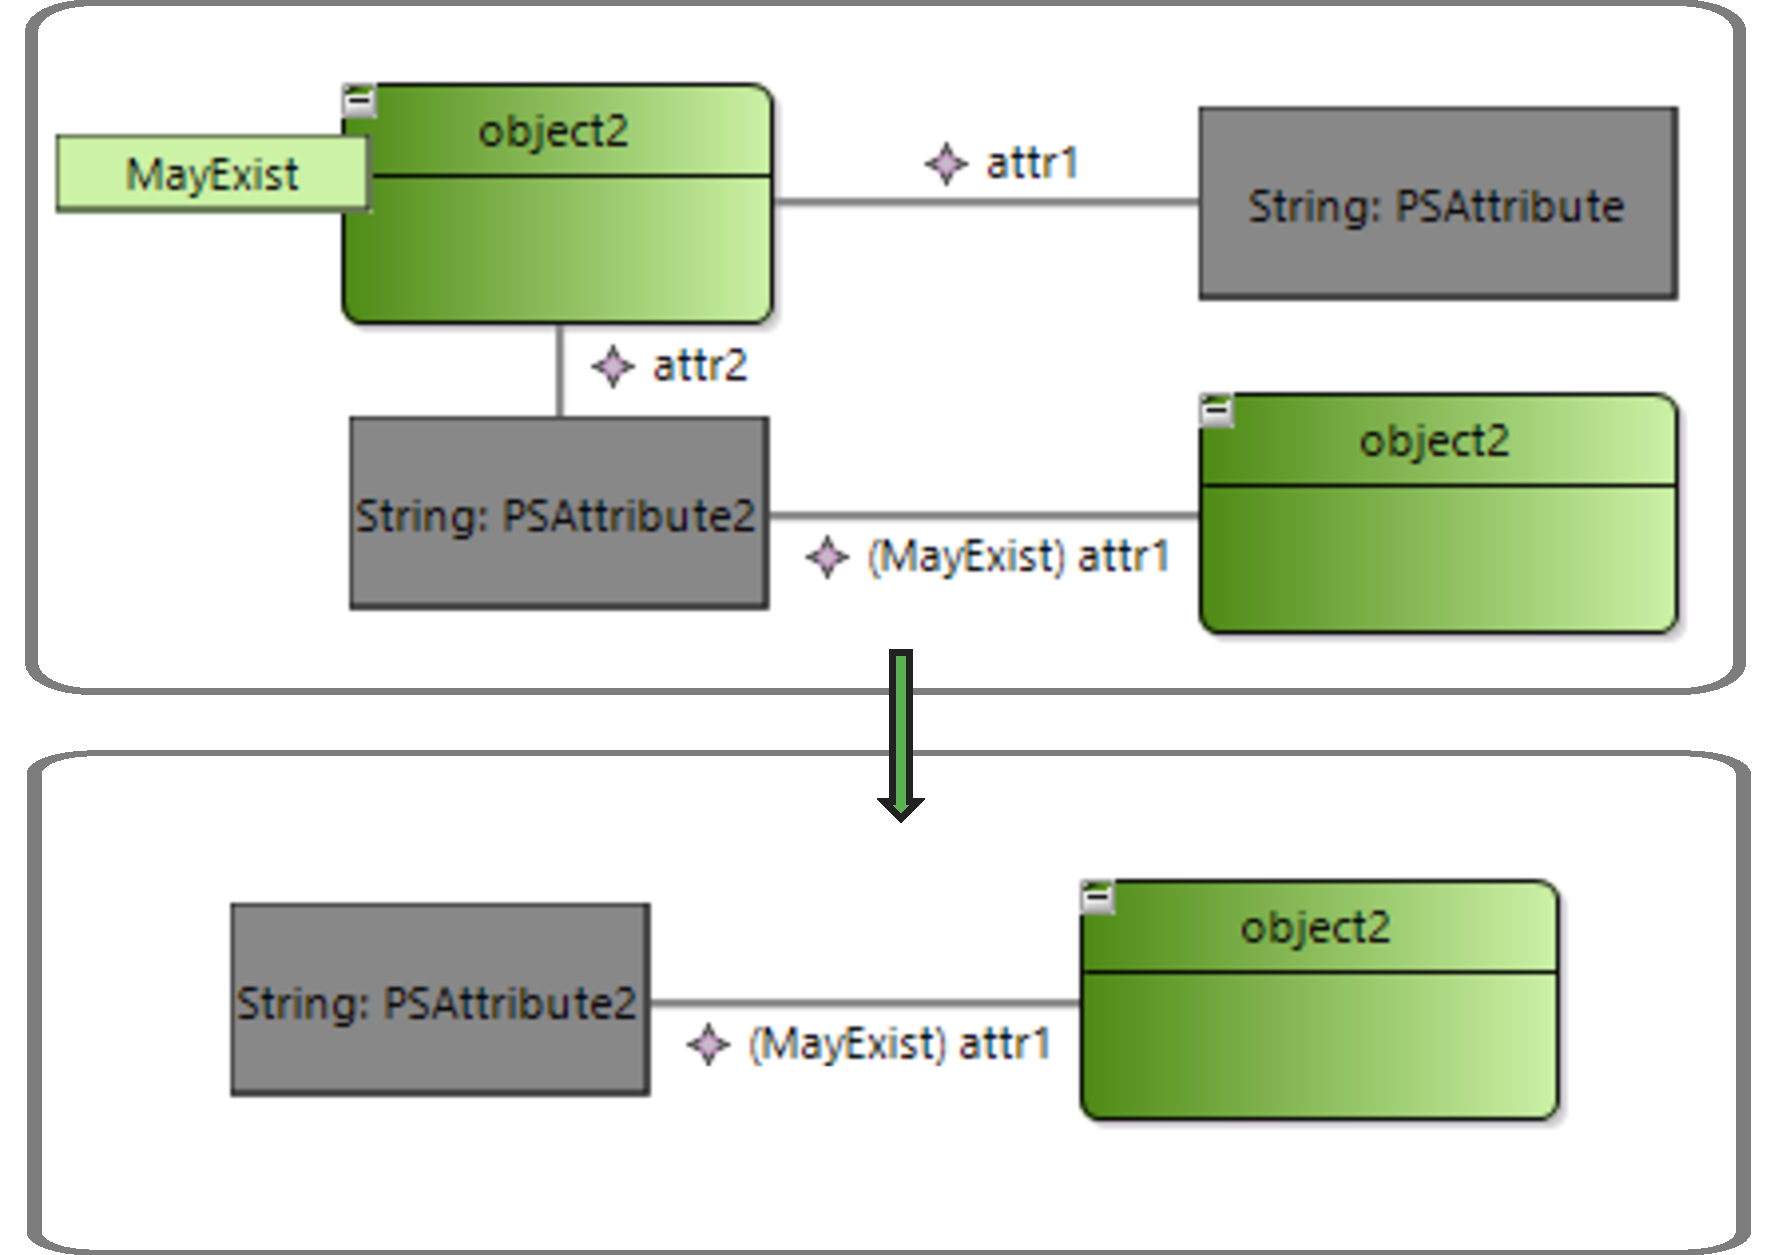
\includegraphics[width=100mm]{figures/objmay.pdf}
	\caption{PSObject finomítása (May)}
	\label{objmay} 
\end{figure}

\subsubsection{PSAttribute-May részlegesség feloldása}
Élek nem törlődnek automatikusan mert a PSObject tartalmazza őket. Végig kell iterálni az összes attribútumra mutató élen és kitörölni azokat. Ezután kitörlődik az attribútum is (lásd \autoref{attrmay}). 
\begin{figure}[!ht]
	\centering
	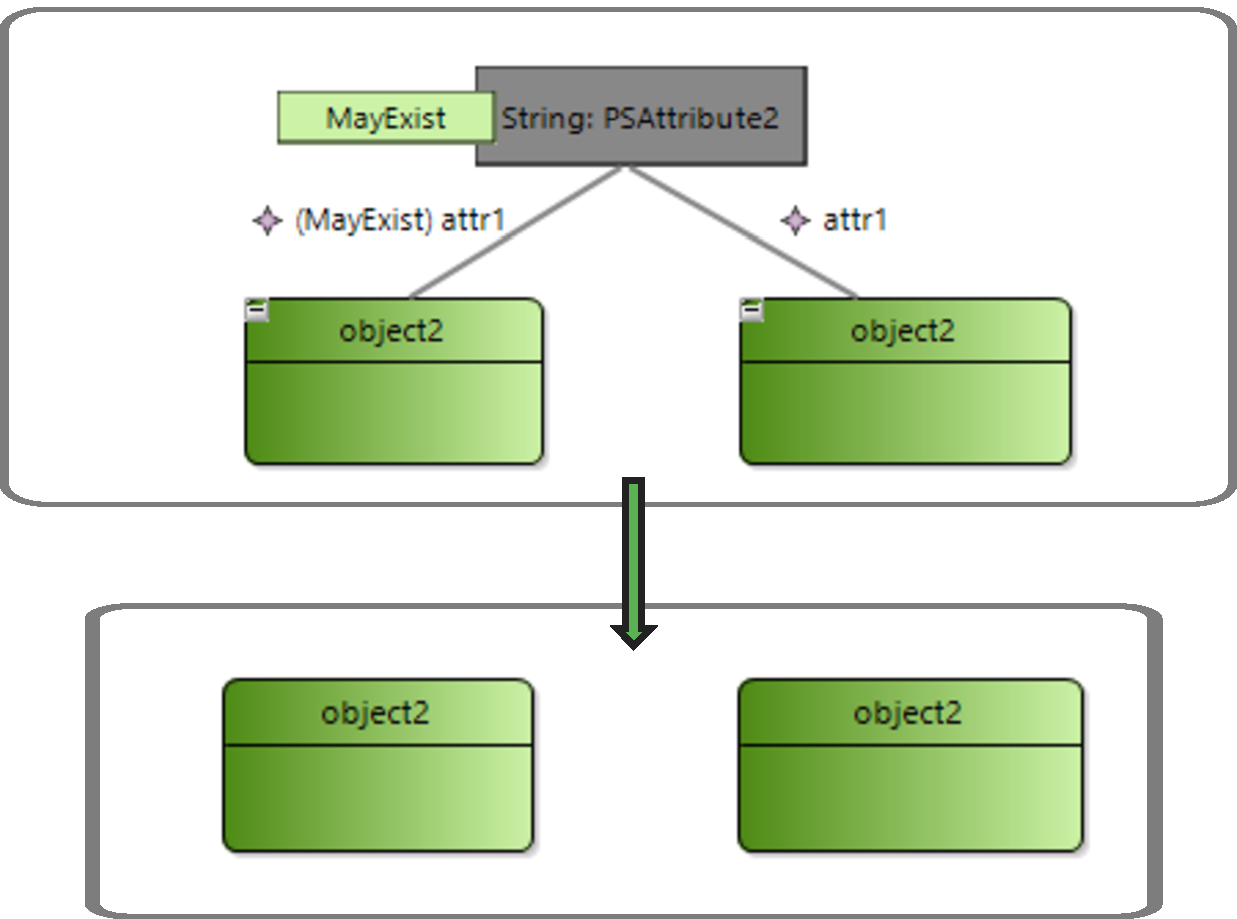
\includegraphics[width=100mm]{figures/attrmay.pdf}
	\caption{PSAttribute finomítása (May)}
	\label{attrmay} 
\end{figure}

\subsubsection{PSReferenceToObject-May részlegesség feloldása}
Kitörli a referenciát a forrásobjektumból.

\subsubsection{PSReferenceToAttribute-May részlegesség feloldása}
Az él törlődik, de eltérően az PSObject-ekre mutató élektől, amennyiben a célattribútumba nem vezet másik él, akkor az attribútum is megszűnik. A finomítás lényege, hogy általa csökken a részlegessége a modellnek. Azért nem lenne értelme az üresen maradt attribútumot meghagyni, ami nem kötődik semmilyen objektumhoz, mert nem csökkent volna a modell részlegessége (lásd \autoref{refmay}).
\begin{figure}[!ht]
	\centering
	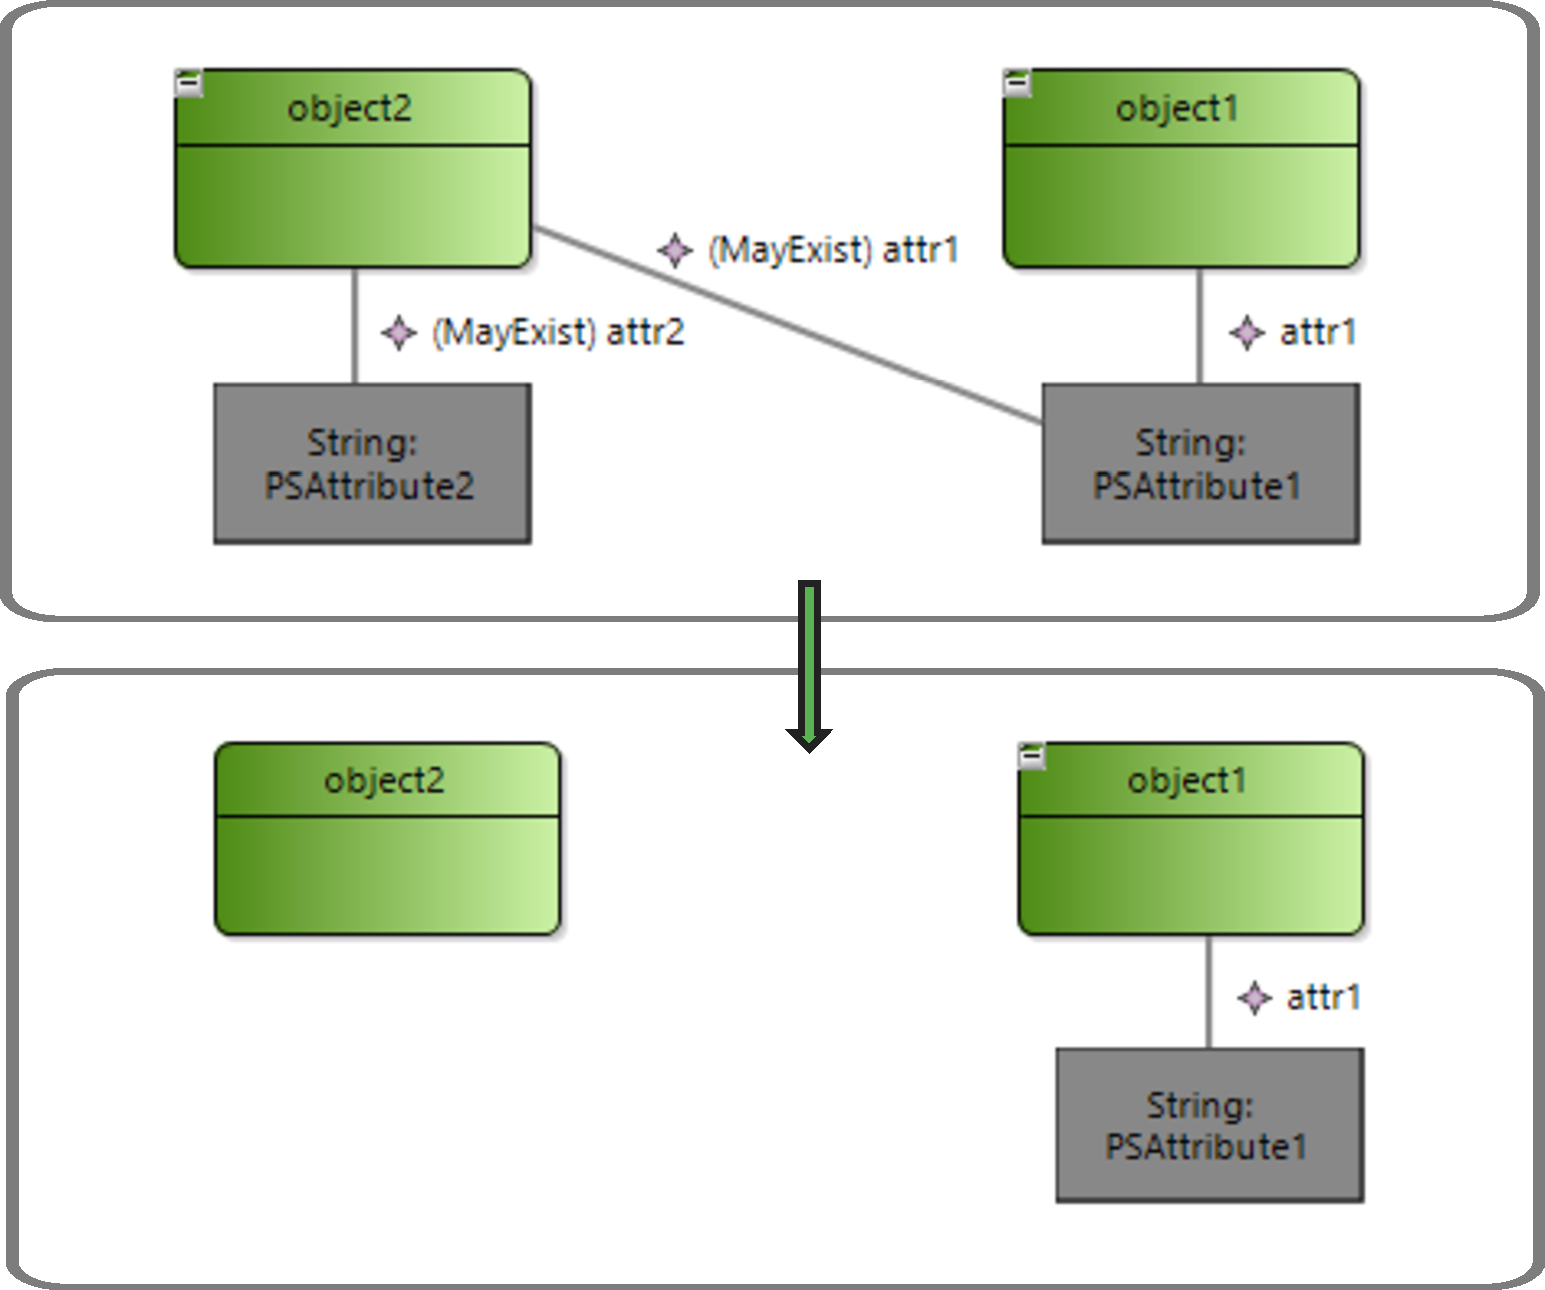
\includegraphics[width=100mm]{figures/refmay.pdf}
	\caption{PSReferenceToAttribute finomítása (May)}
	\label{refmay} 
\end{figure}

\subsubsection{PSObject-Set részlegesség feloldása}
Létrejön egy új objektum, aminek ugyanazok a tulajdonságai, mint az eredeti objektumnak, amin a 'Set' annotáció volt. Az új PSObject referenciái ugyan azokra az objektumokra mutatnak, mint az eredeti PSObject esetében. Új attribútumok jönnek létre az eredeti objektumhoz tartozó attribútumok mintájára és ezek lesznek összekötve az új PSObject-el. Az új élek nevei ugyan azok mint az eredeti esetben, de a végére kerül egy kis 'v' betű (lásd \autoref{objset}).
\begin{figure}[!ht]
	\centering
	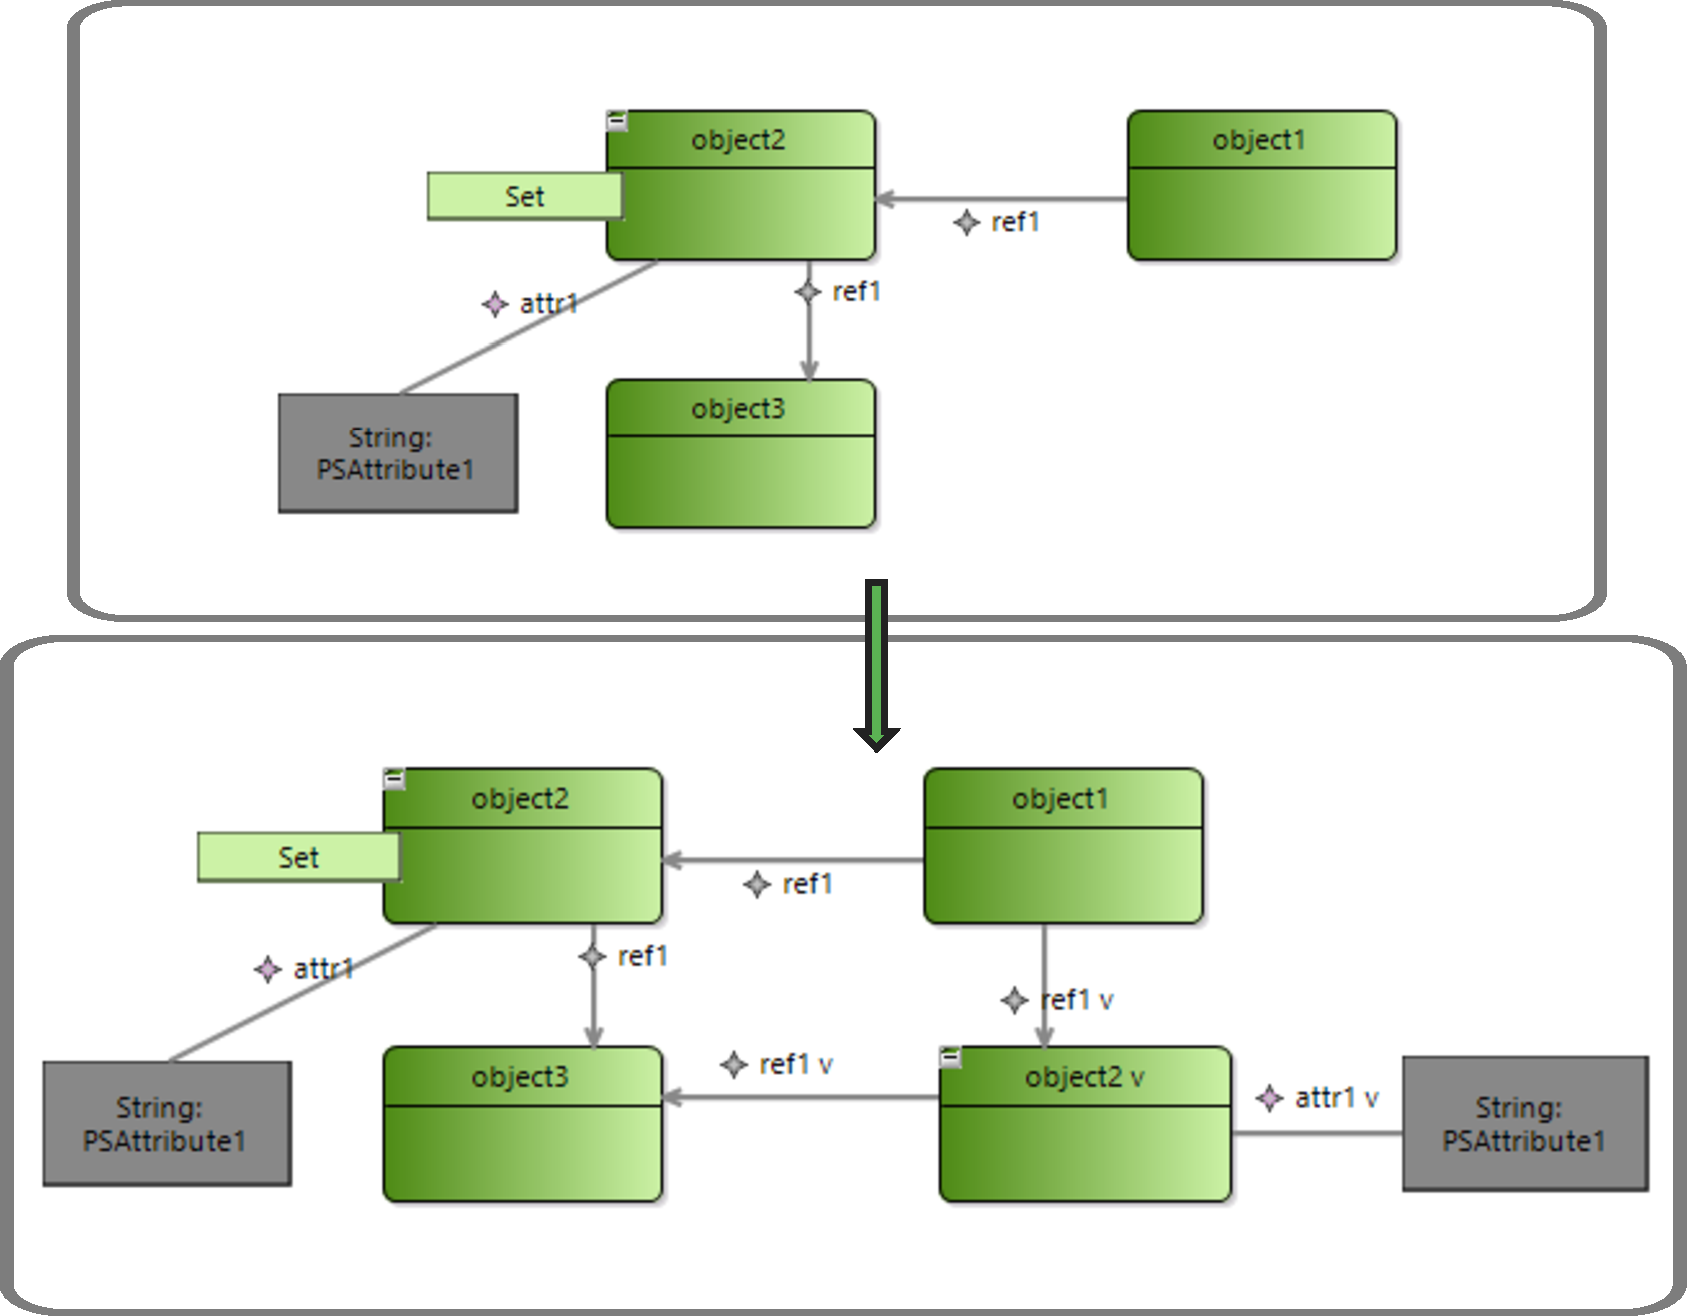
\includegraphics[width=100mm]{figures/objset.pdf}
	\caption{PSObject finomítása (Set)}
	\label{objset} 
\end{figure}

\subsubsection{PSAttribute-Set részlegesség feloldása}
Létrejön egy új attribútum és ugyan ahhoz az PSObject-hez fog tartozni mint az eredeti,  tehát az objektumból él fog vezetni az attribútumba. A típusát és értékét is megörökli az eredeti attribútumnak. Új elemhez tartozó referenciák nevei után egy kis 'v' betű kerül (lásd \autoref{attrset}).
\begin{figure}[!ht]
	\centering
	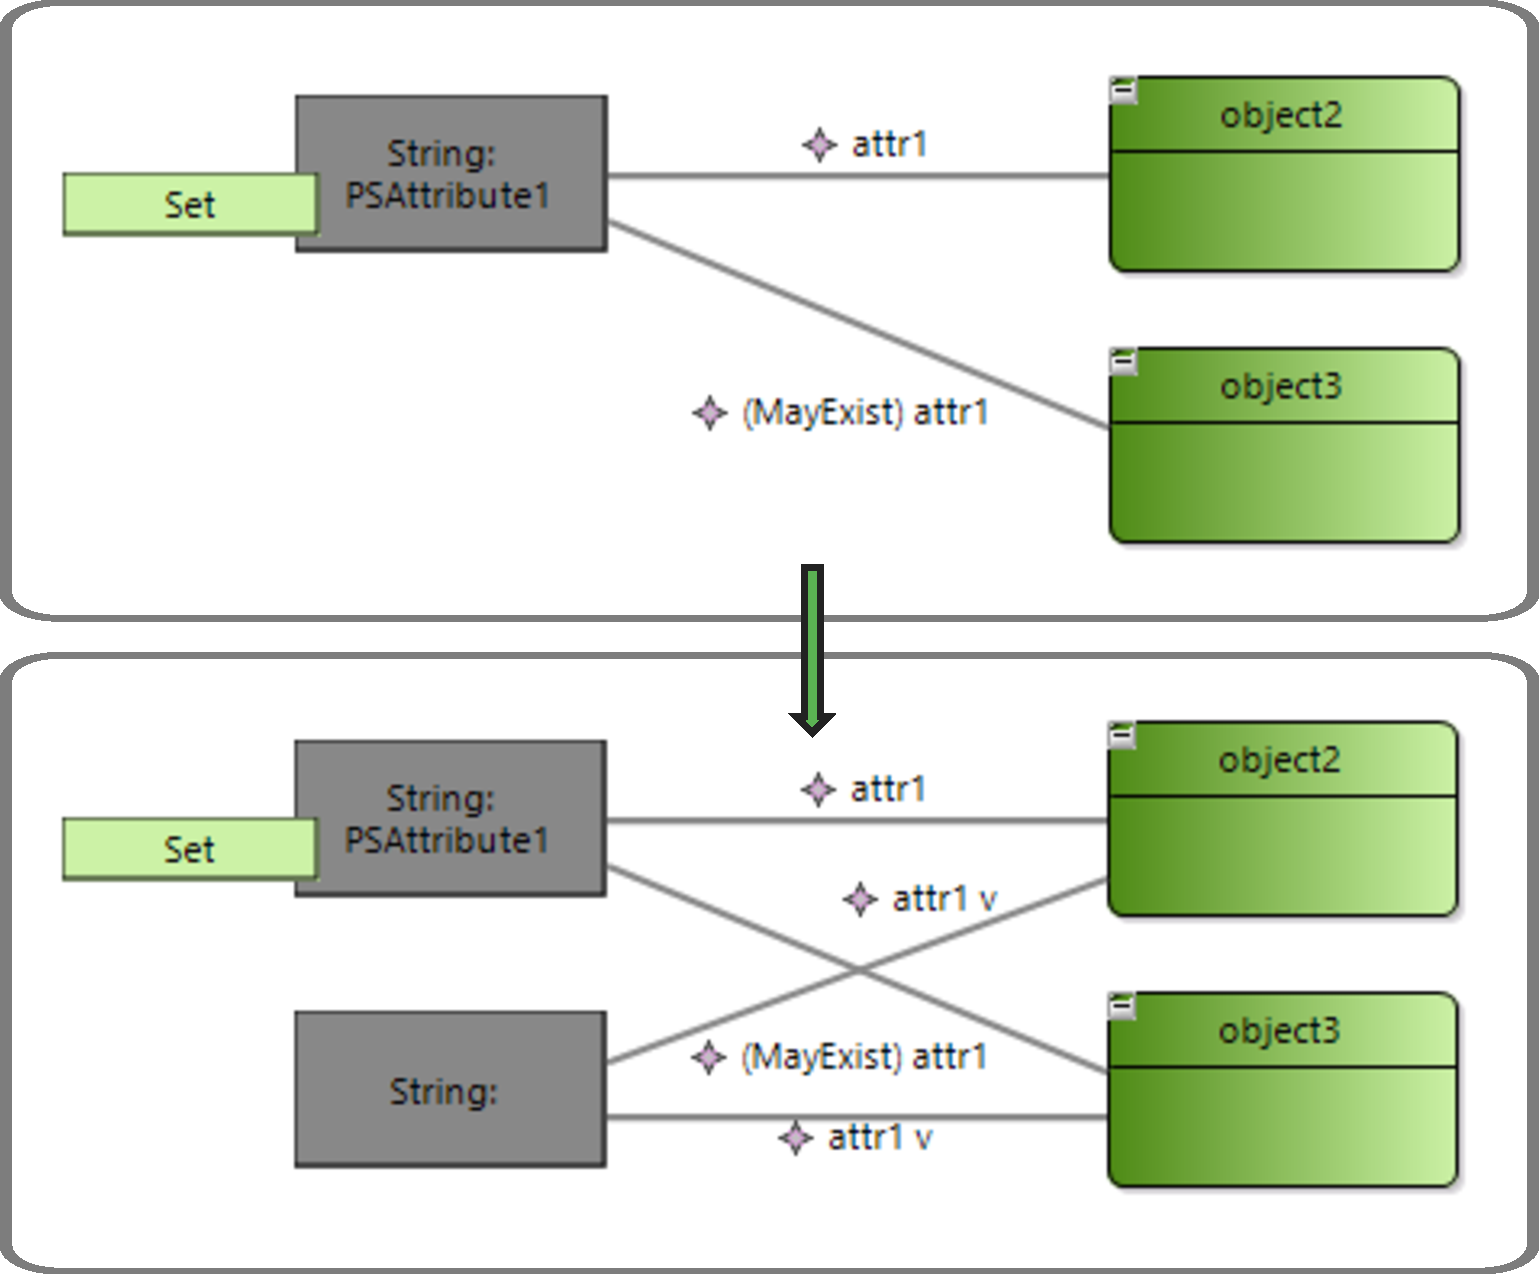
\includegraphics[width=100mm]{figures/attrset.pdf}
	\caption{PSAttribute finomítása (Set)}
	\label{attrset} 
\end{figure}

\subsubsection{PSReferenceToObject-Set részlegesség feloldása}
Az eredeti referencia forrásobjektumában létrehoz egy újat, ami ugyan arra az objektumra mutat (lásd \autoref{refset}).

\subsubsection{PSReferenceToAttribute-Set részlegesség feloldása}
Az eredeti referencia forrásobjektumában létrehoz egy újat, ami ugyan arra az attribútumra mutat, ezután a célattribútum referenciái közé is hozzáadjuk az új élet(lásd \autoref{refset}).
\begin{figure}[!ht]
	\centering
	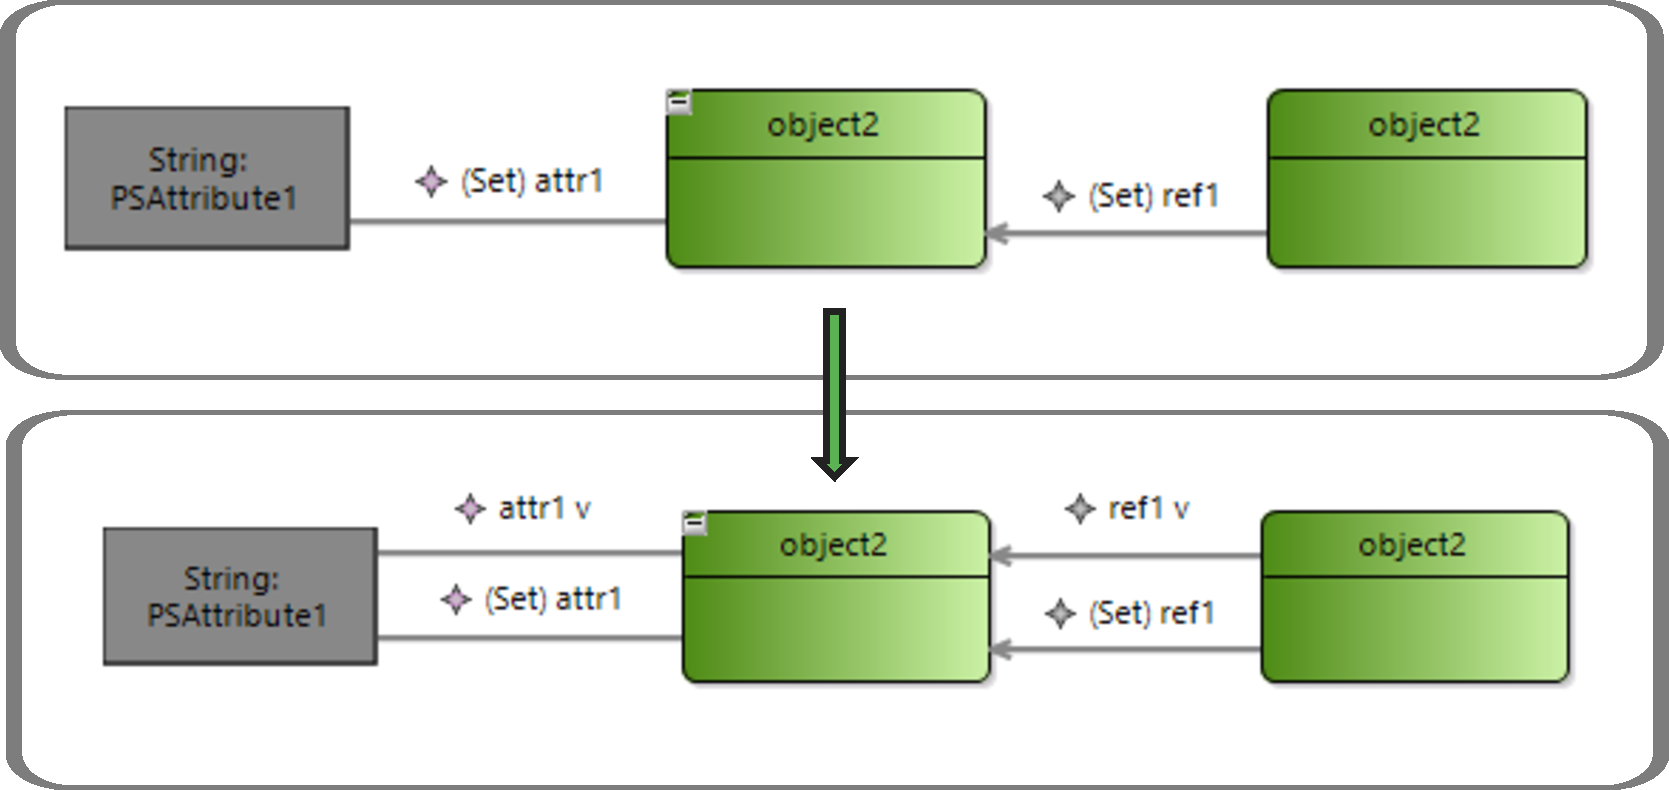
\includegraphics[width=100mm]{figures/refset.pdf}
	\caption{PSReference finomítása (Set)}
	\label{refset} 
\end{figure}

\subsubsection{Var részlegességről általában}
Eredeti objektumnak, elemnek nevezem a továbbiakban azt a PSObject-et amelyiknél a 'Var' részlegességére duplán kattintottunk. A 'Var' részlegességnek van egy id-ja, ami segítségével meg lehet jelölni, hogy melyik 'Var' részlegességek tartoznak egybe, erre a későbbiekben 'Var id'-val hivatkozom.


\subsubsection{PSObject-Var részlegesség feloldása}
 Az összes olyan objektumnak, amelyiknek megegyezik a 'Var id'-ja az törlődik, kivéve az eredeti de előtte az összes hozzá tartozó referencia mintájára létrejönnek az eredeti objektumban élek. Azok az objektumok élei, amik eddig egy törölt objektumba mutattak, azok most az eredeti objektumra fognak mutatni (lásd \autoref{objvar}).
\begin{figure}[!ht]
	\centering
	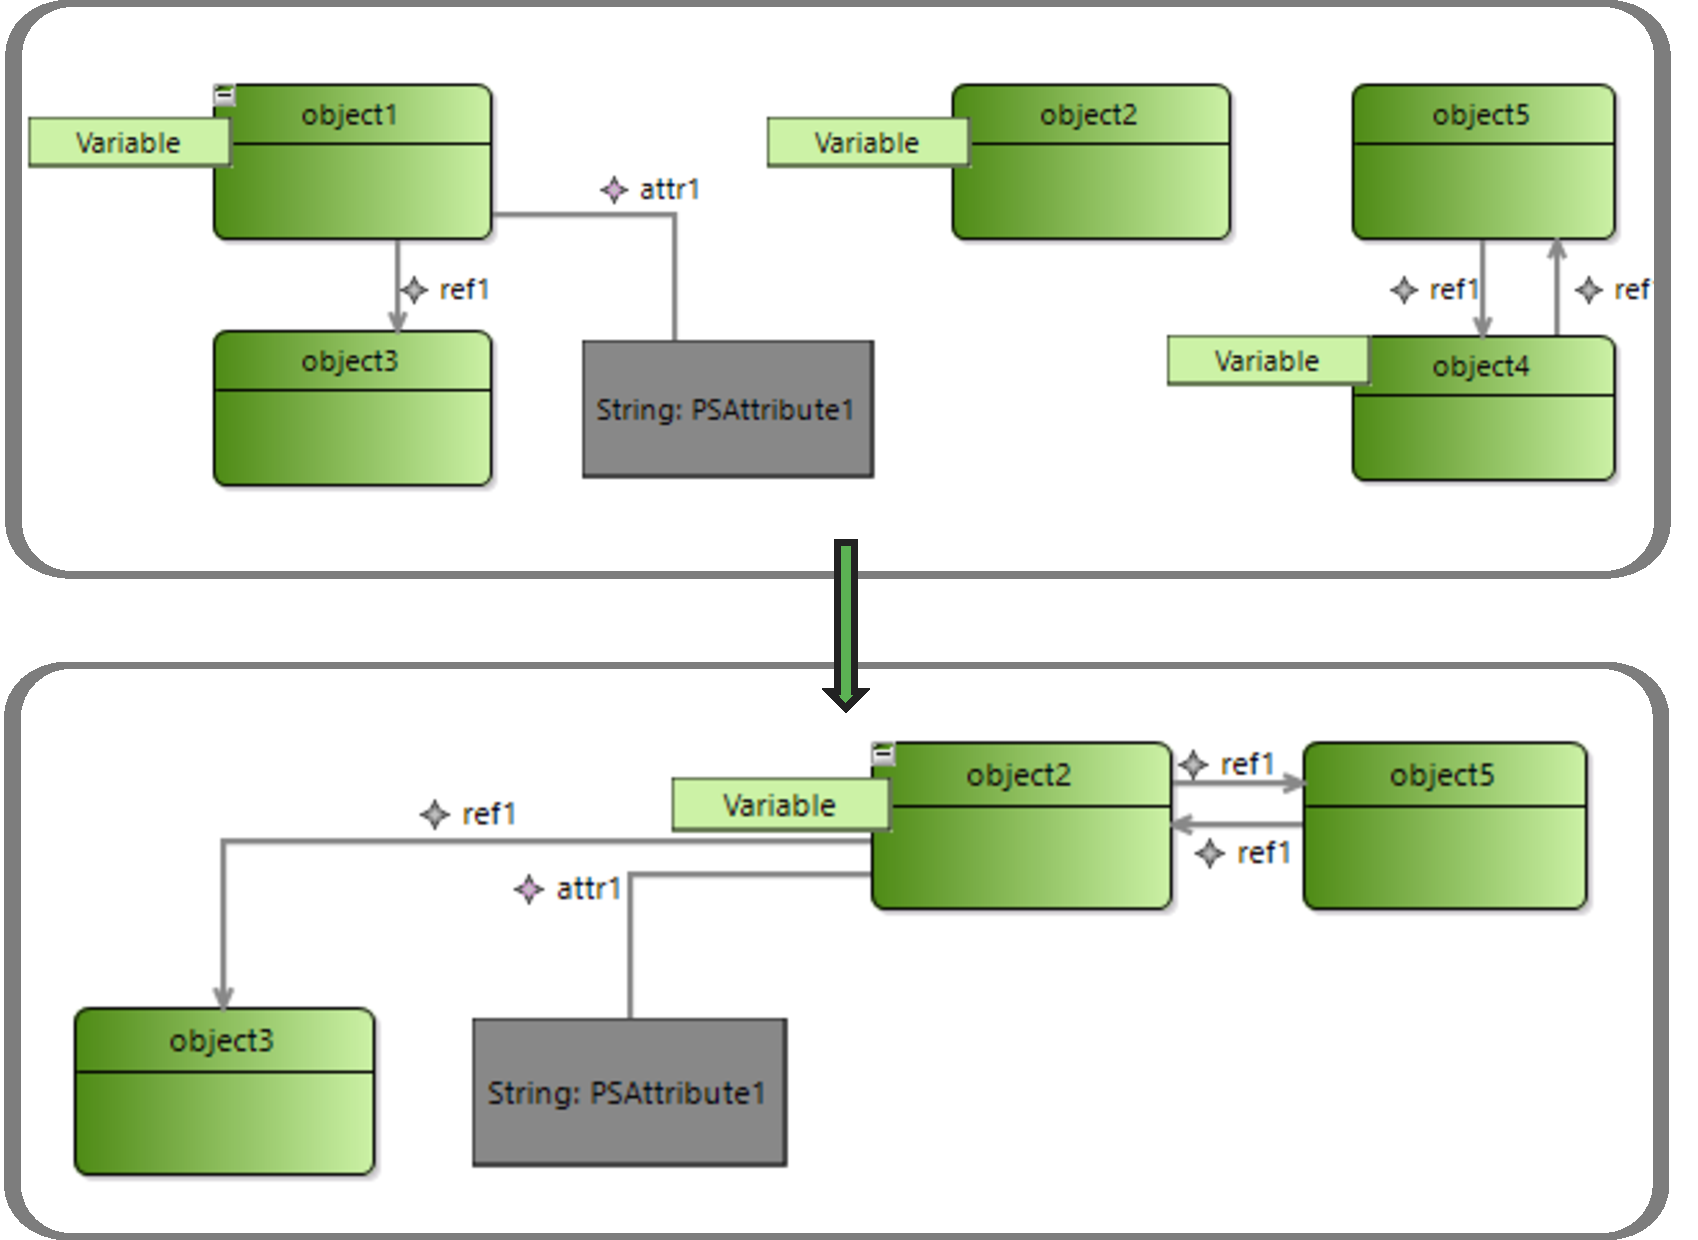
\includegraphics[width=110mm]{figures/objvar.pdf}
	\caption{PSObject finomítása (Var)}
	\label{objvar} 
\end{figure}

\subsubsection{PSAttribute-Var részlegesség feloldása}
Az eredetin kívül az összes olyan attribútum kitörlődik, aminek a 'Var id'-ja megegyezik az eredeti elem 'Var id'-jával. A törölt elemekbe futó élek az eredeti elemre fognak ezentúl mutatni (lásd \autoref{attrvar}).
\begin{figure}[!ht]
	\centering
	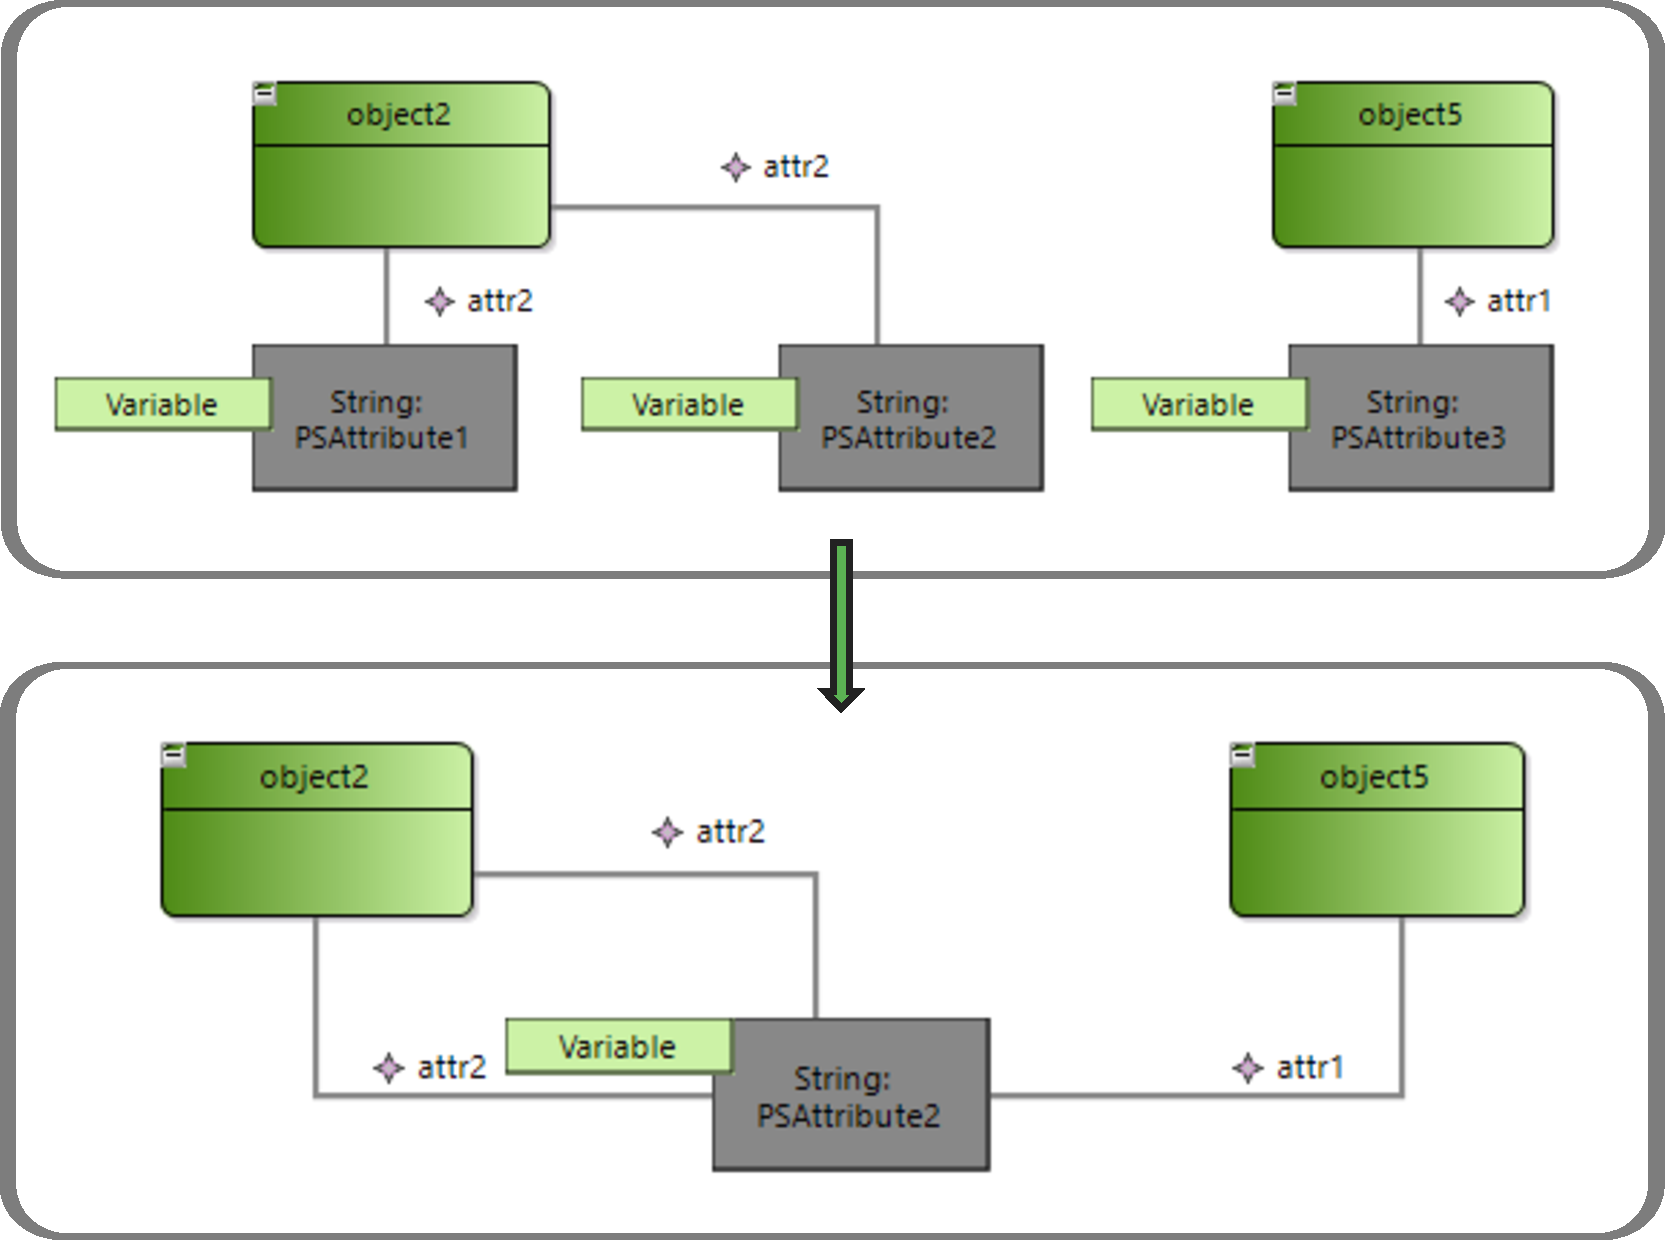
\includegraphics[width=110mm]{figures/attrvar.pdf}
	\caption{PSAttribute finomítása (Var)}
	\label{attrvar} 
\end{figure}

\subsubsection{PSReferenceToObject-Var részlegesség feloldása}
Csak az eredeti referencia forrásobjektumában keres vele megegyező 'Var id'-val rendelkező referenciát. Ezeket a referenciákat törli (lásd \autoref{refvar}).


\subsubsection{PSReferenceToAttribute-Var részlegesség feloldása}
Hasonlóan a PSReferenceToObject esetéhez csak az eredeti referencia forrásobjektumában keres vele megegyező 'Var id'-val rendelkező referenciát. Ezeket a referenciákat törli (lásd \autoref{refvar}).

\begin{figure}[!ht]
	\centering
	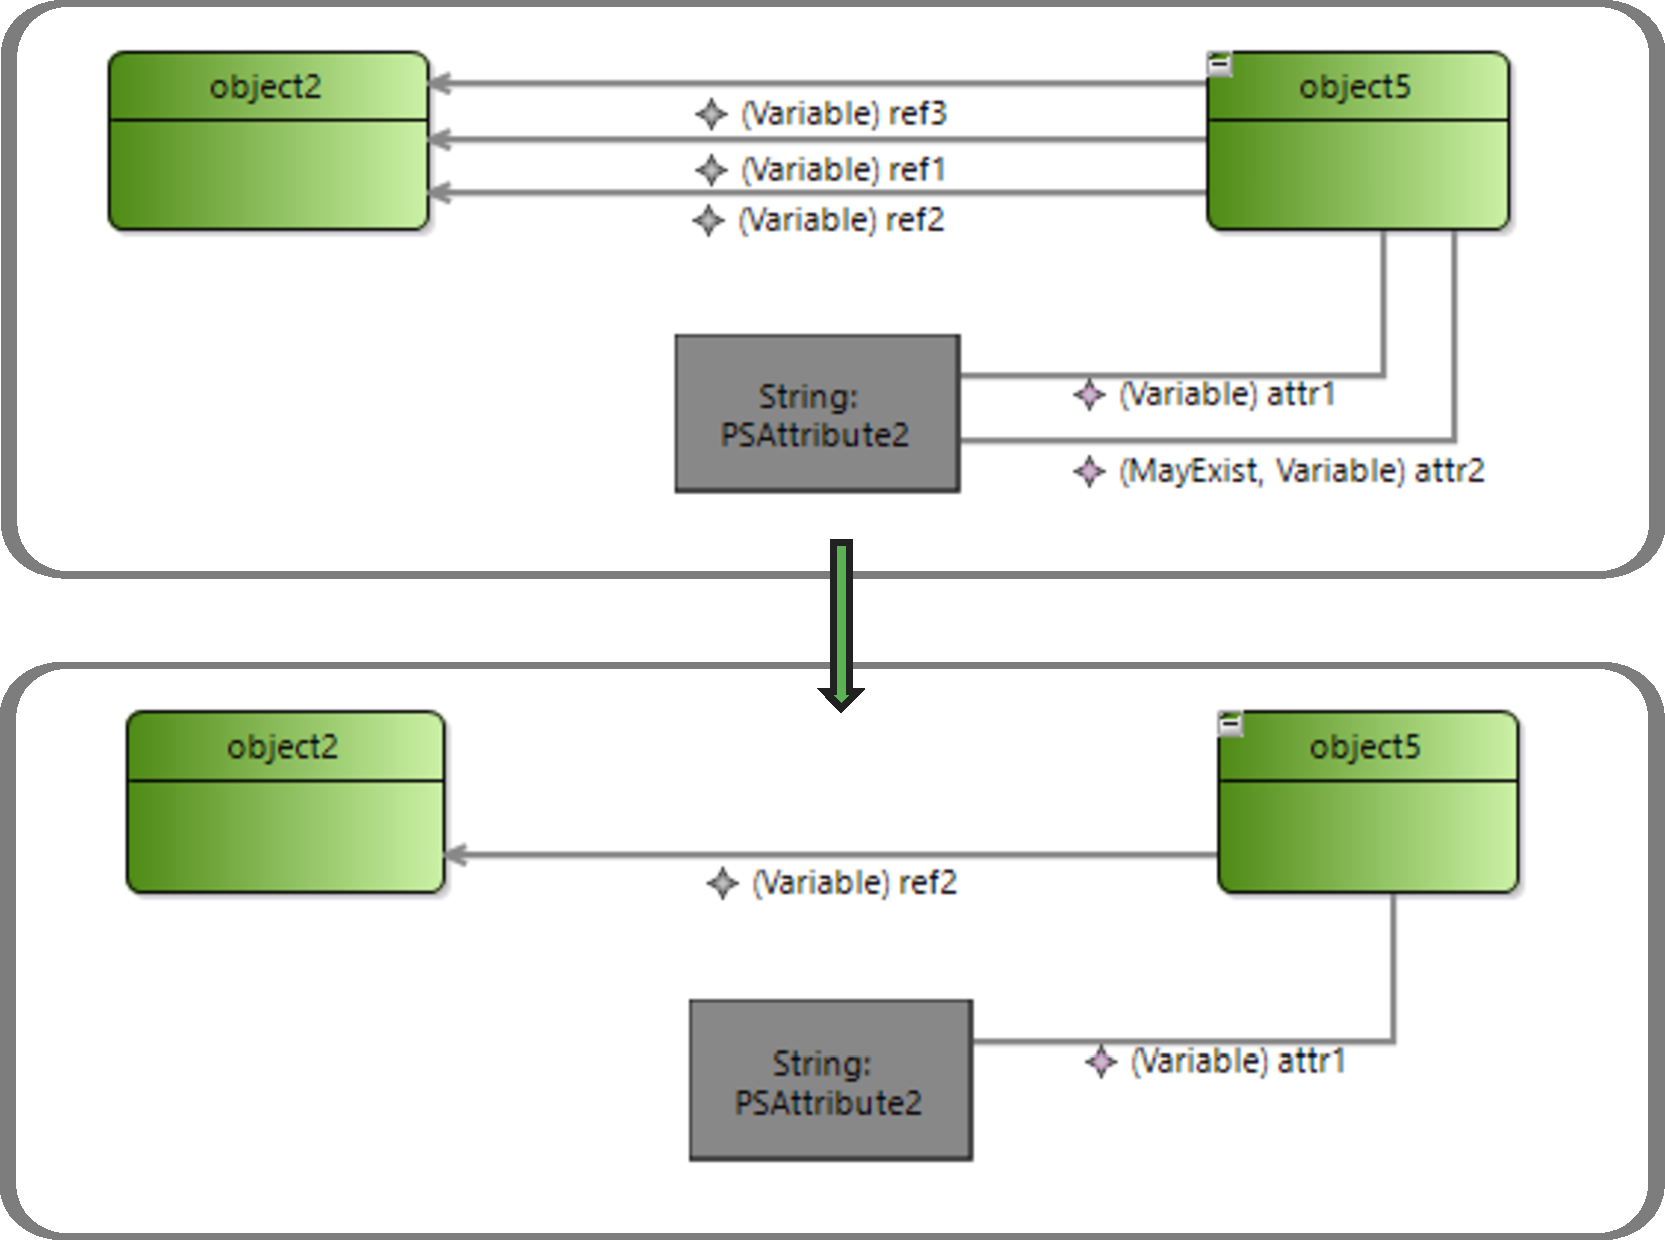
\includegraphics[width=110mm]{figures/refvar.pdf}
	\caption{OSReference finomítása (Var)}
	\label{refvar} 
\end{figure}
%----------------------------------------------------------------------------
\chapter{Összefoglalás és továbbfejlesztési lehetőségek}\label{chapter:summary}
%----------------------------------------------------------------------------
Dolgozatom során elkészítettem egy általános célú modellezési nyelvet, melynek segítségével parciális modelleket lehet készíteni. Ehhez tartozik egy szerkesztőfelület, ami támogatja ezen modellek módosítását, fejlesztését. Lehet benne objektumokat, attribútumokat és referenciákat létrehozni. Objektumok tartalmazhatnak attribútumokat és referenciák segítségével kapcsolódhatnak más objektumokhoz. Attribútumok függetlenül is létezhetnek az objektumtól. A felsorolt három elem mindegyikéhez lehetséges részlegességeket rendelni: 'May', 'Var', 'Abs'. Magát a modellt pedig meg lehet jelölni 'OW' részlegességgel. A modellt finomítani lehet, mely során csökkenthető annak részlegessége. Ezen részlegességek feloldása a részlegességek szemantikájától függően történik.
\par
A részleges modellek vizsgálatát rengeteg más szemszögből is meg lehet közelíteni. Lehetséges a szerkesztőt továbbfejleszteni, új funkciókkal és validációkkal bővíteni. Jelenleg a modellező eszközben tudunk készíteni parciális modelleket, de már meglévő modellek szerkesztése részleges modellként nem lehetséges. Erre lehetne készíteni egy programot, ami szerkeszteni kívánt modell minden elemét megfelelteti egy parciális modellbeli elemmel. Így például a dolgozatban szereplő jármű (lásd \autoref{jarmu}) minden objektumát "becsomagolhatjuk" agy részleges modellhez tartozó objektumba. Ezután ez az elkészített szerkesztőben módosítható. Amennyiben nem kívánunk változtatni a modell egy hasonló programmal visszaalakítható lehet. Ezen a szálon tovább haladva lehetne részlegességet tartalmazó modellből is generálni az importálthoz hasonló modellt. A generáló program többféle modellt készíthet a parciális modellből, figyelembe véve, hogy milyen részlegességeket tartalmaz.




% Acknowledgements
%~~~~~~~~~~~~~~~~~~~~~~~~~~~~~~~~~~~~~~~~~~~~~~~~~~~~~~~~~~~~~~~~~~~~~~~~~~~~~~~~~~~~~~
%\include{content/acknowledgement}


% List of Figures, Tables
%~~~~~~~~~~~~~~~~~~~~~~~~~~~~~~~~~~~~~~~~~~~~~~~~~~~~~~~~~~~~~~~~~~~~~~~~~~~~~~~~~~~~~~
%\listoffigures\addcontentsline{toc}{chapter}{\abrakjegyzeke}
%\listoftables\addcontentsline{toc}{chapter}{\tablazatokjegyzeke}


% Bibliography
%~~~~~~~~~~~~~~~~~~~~~~~~~~~~~~~~~~~~~~~~~~~~~~~~~~~~~~~~~~~~~~~~~~~~~~~~~~~~~~~~~~~~~~
\bibliography{bib/mybib}
\addcontentsline{toc}{chapter}{\irodalomjegyzek}


% Appendix
%~~~~~~~~~~~~~~~~~~~~~~~~~~~~~~~~~~~~~~~~~~~~~~~~~~~~~~~~~~~~~~~~~~~~~~~~~~~~~~~~~~~~~~
%\include{content/appendices}

%\label{page:last}
\end{document}
